\documentclass[10pt,a4paper,twocolumn]{article}
\usepackage{graphicx} 
\usepackage[labelformat=empty]{caption}
\usepackage{import}
\usepackage[T2A]{fontenc}
\usepackage[margin=1.5cm,top=1.5cm]{geometry}
\usepackage[english,russian]{babel}
\title {\textbf{Pасчетная работа}}
\author{Рассохов Егор 421703}
\date{}
\begin{document}
\maketitle
\large{\hspace{-0.4cm}\textbf{Цель:}}
\par Продемонстрировать работу программы решения теоретико-графовой задачи по построению конденсированного графа для орграфа
\\ \large{\textbf {Ключевые понятия:}}
\par Граф – математическая абстракция реальной системы любой природы, объекты которой обладают парными связями. Граф как математический объект есть совокупность двух множеств — множества самих объектов, называемого множеством вершин, и множества их парных связей, называемого множеством рёбер. 
\par Ориентированный граф (кратко орграф) — граф, рёбра которого имеют направление.
\par Путь в графе – это последовательность рёбер, в которой конец каждого ребра (кроме последнего) совпадает с началом следующего. 
\par Матрица смежности - это вид представления графа в виде матрицы, когда пересечение столбцов и строк задаёт дуги.
\par Компонента сильной связности орграфа - его максимальная по включению сильно связный подграф.
\par Область сильной связности - множество вершин компонентов сильной связности.
\par\large{\hspace{-0.6cm}\textbf{Демонстрация работы программы в семантической памяти на примере невзвешенного ориентированного графа:}}
\par Каждому пункту соответствует рисунок с соответствующим номером.
\begin{enumerate}
% 1
	\item Передаём на вход ориентированный граф.
	\begin{figure}[h!]
		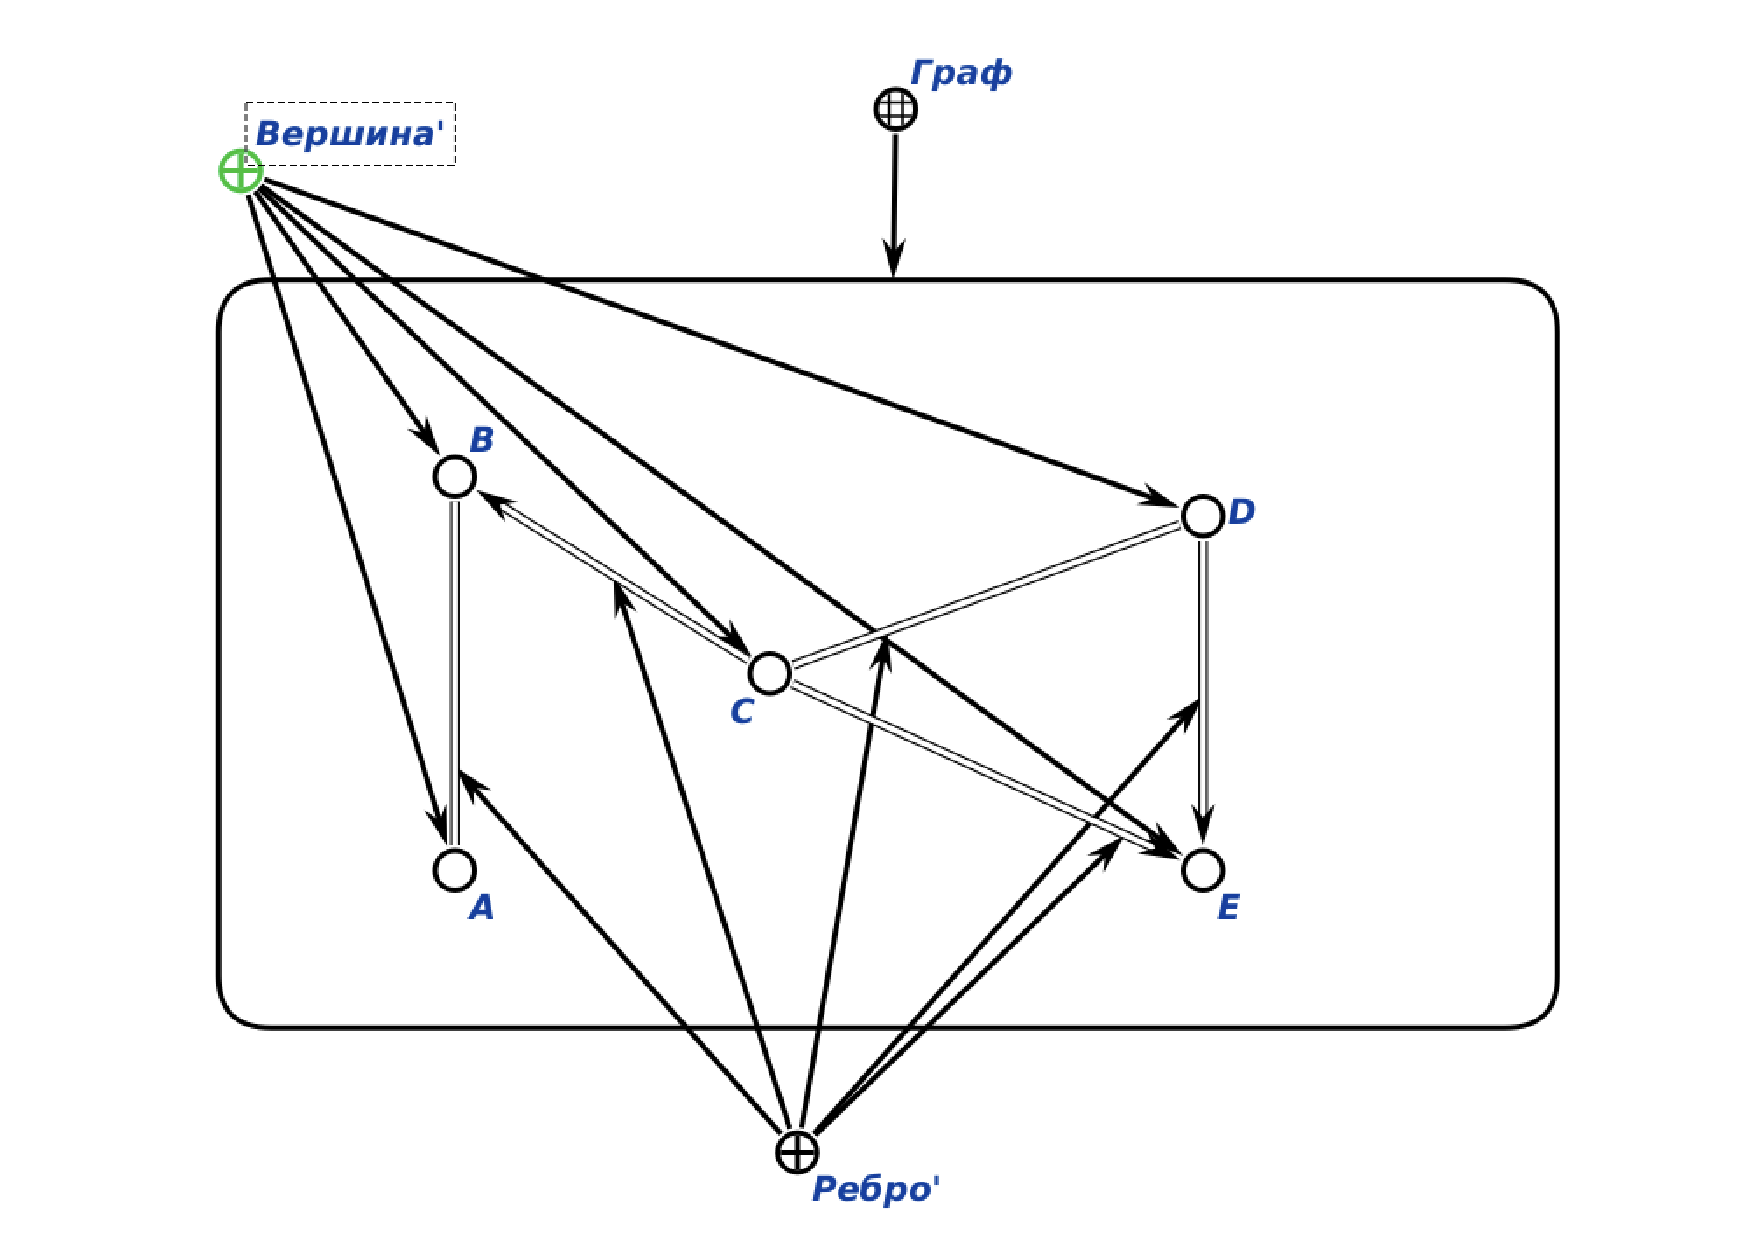
\includegraphics[width=0.5\textwidth]{img/1.png}
		\caption{Рис.1}
	\end{figure}
% 2
	\item Создаём структуры данных для хранения посещённых вершин (посещение) и очередь выхода (очередь), а также текущая и вершина начала обхода.
	\begin{figure}[h!]
		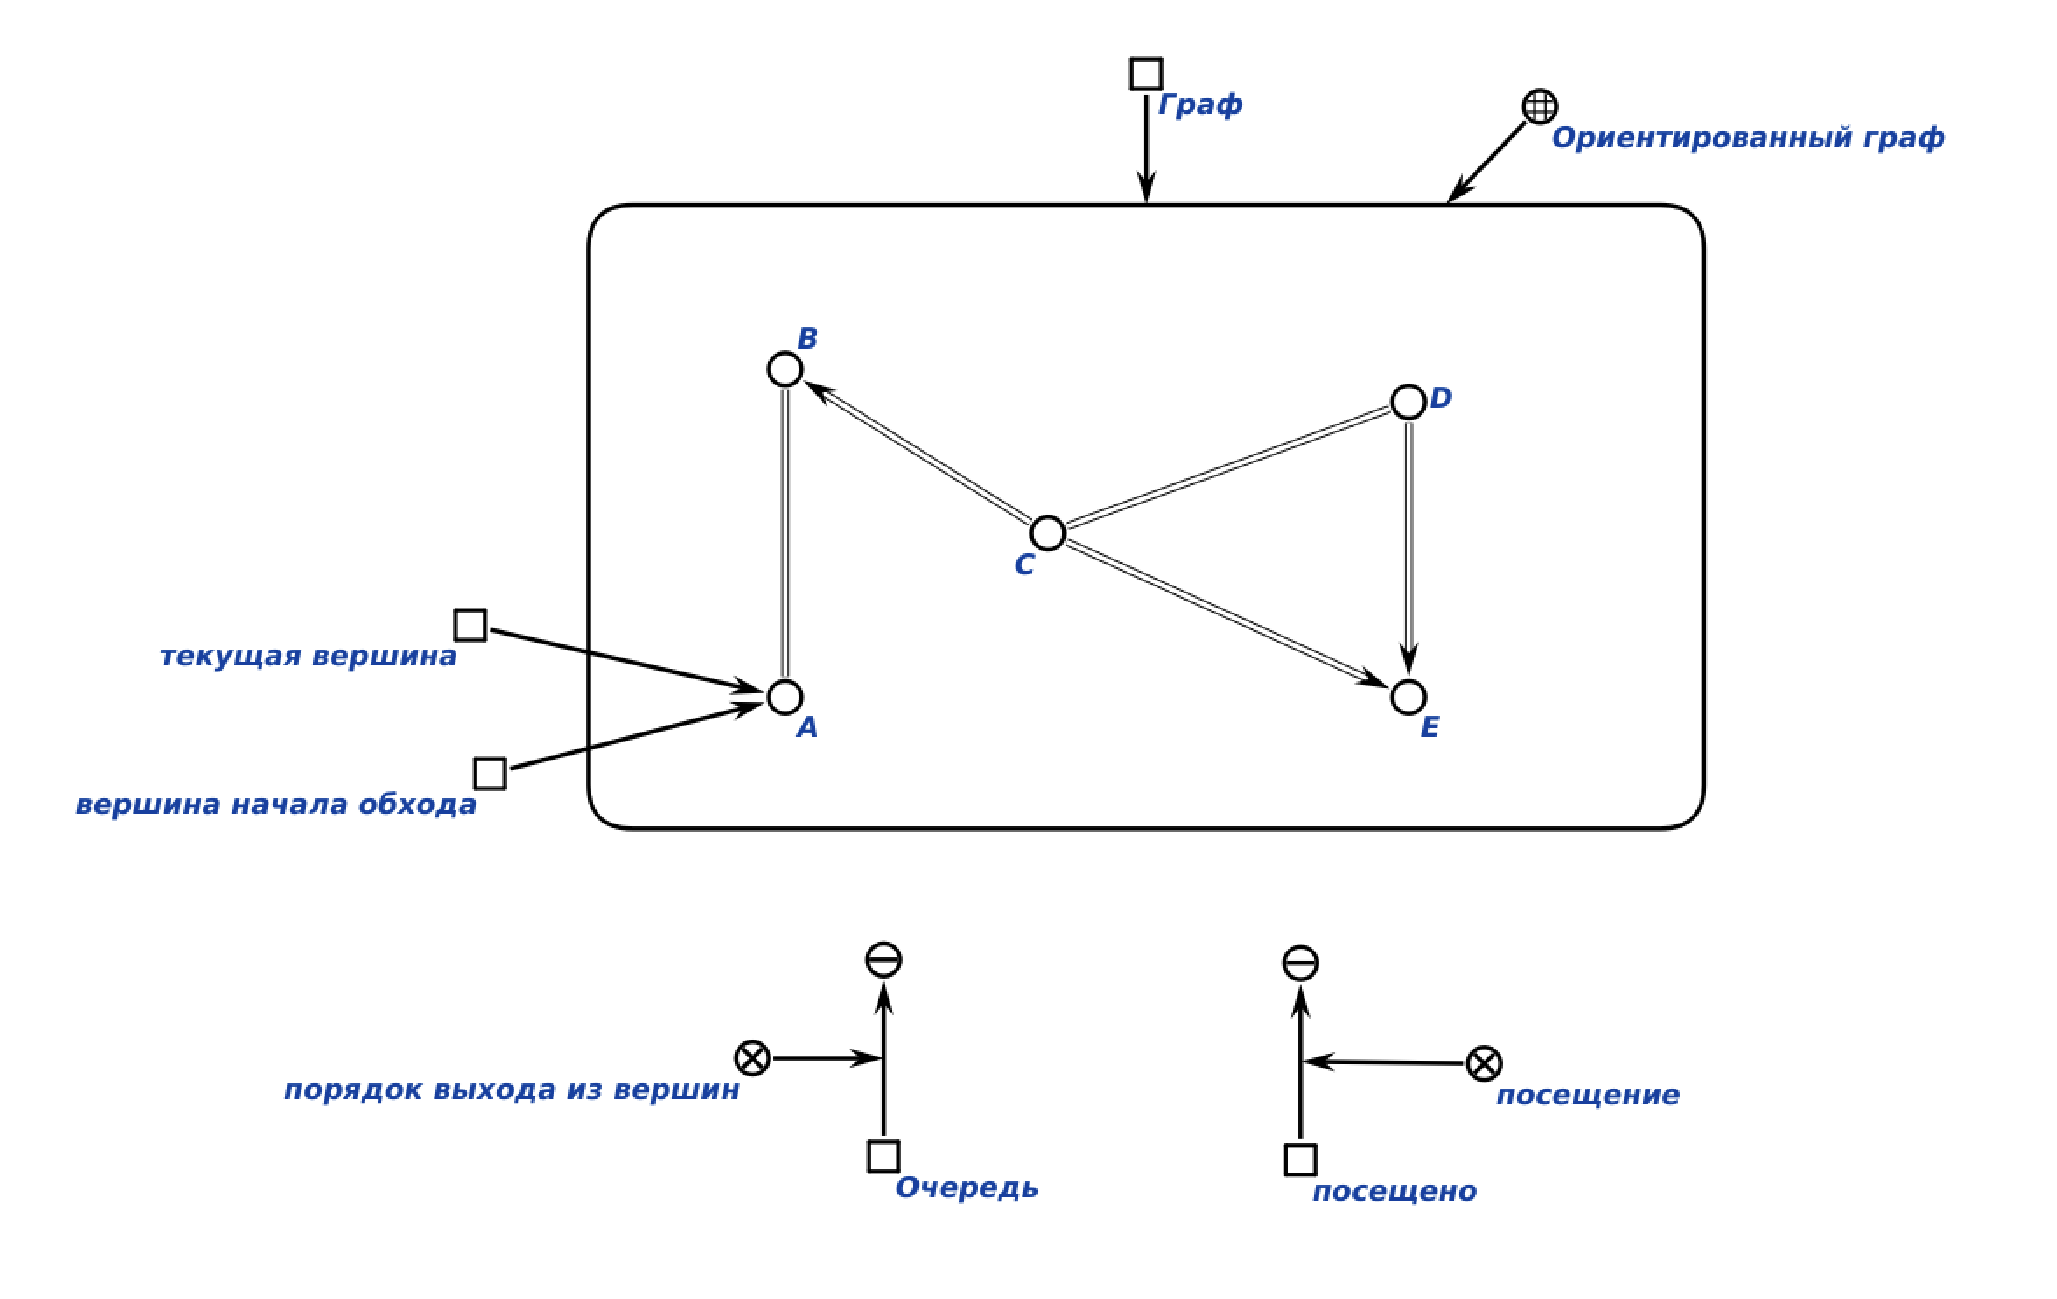
\includegraphics[width=0.5\textwidth]{img/2.png}
		\caption{Рис.2}
	\end{figure}
% 3
	\item Помечаем вершину A как посещённую.
    \begin{figure}[h]
		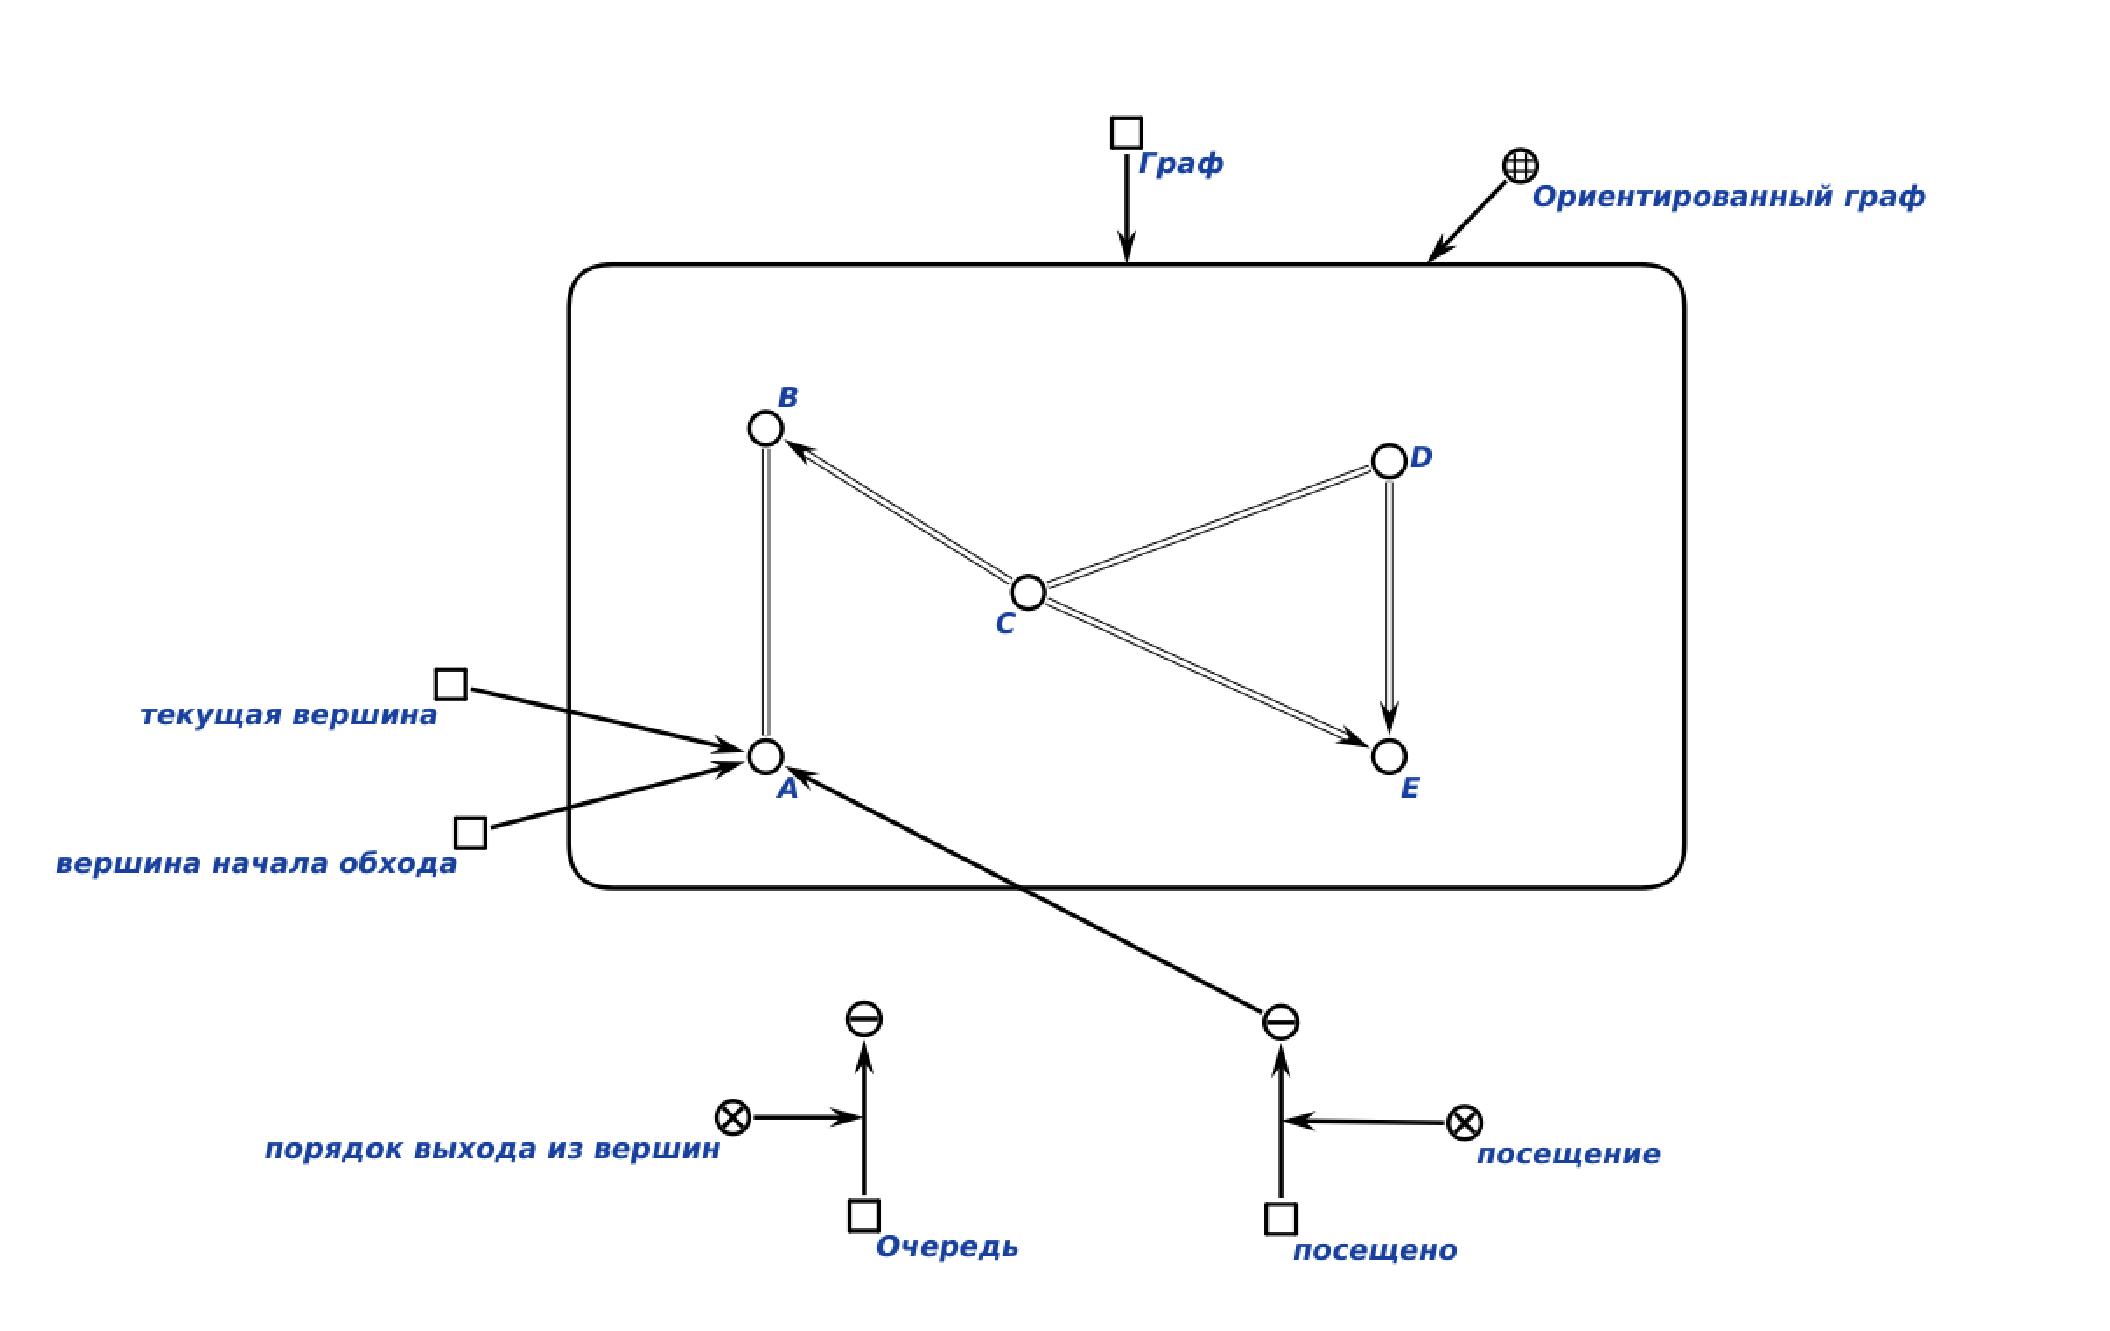
\includegraphics[width=0.45\textwidth]{img/3.png}
		\caption{Рис.3}
	\end{figure}
% 4
	\item Помечаем вершину B как посещённую.
	\begin{figure}[h]
		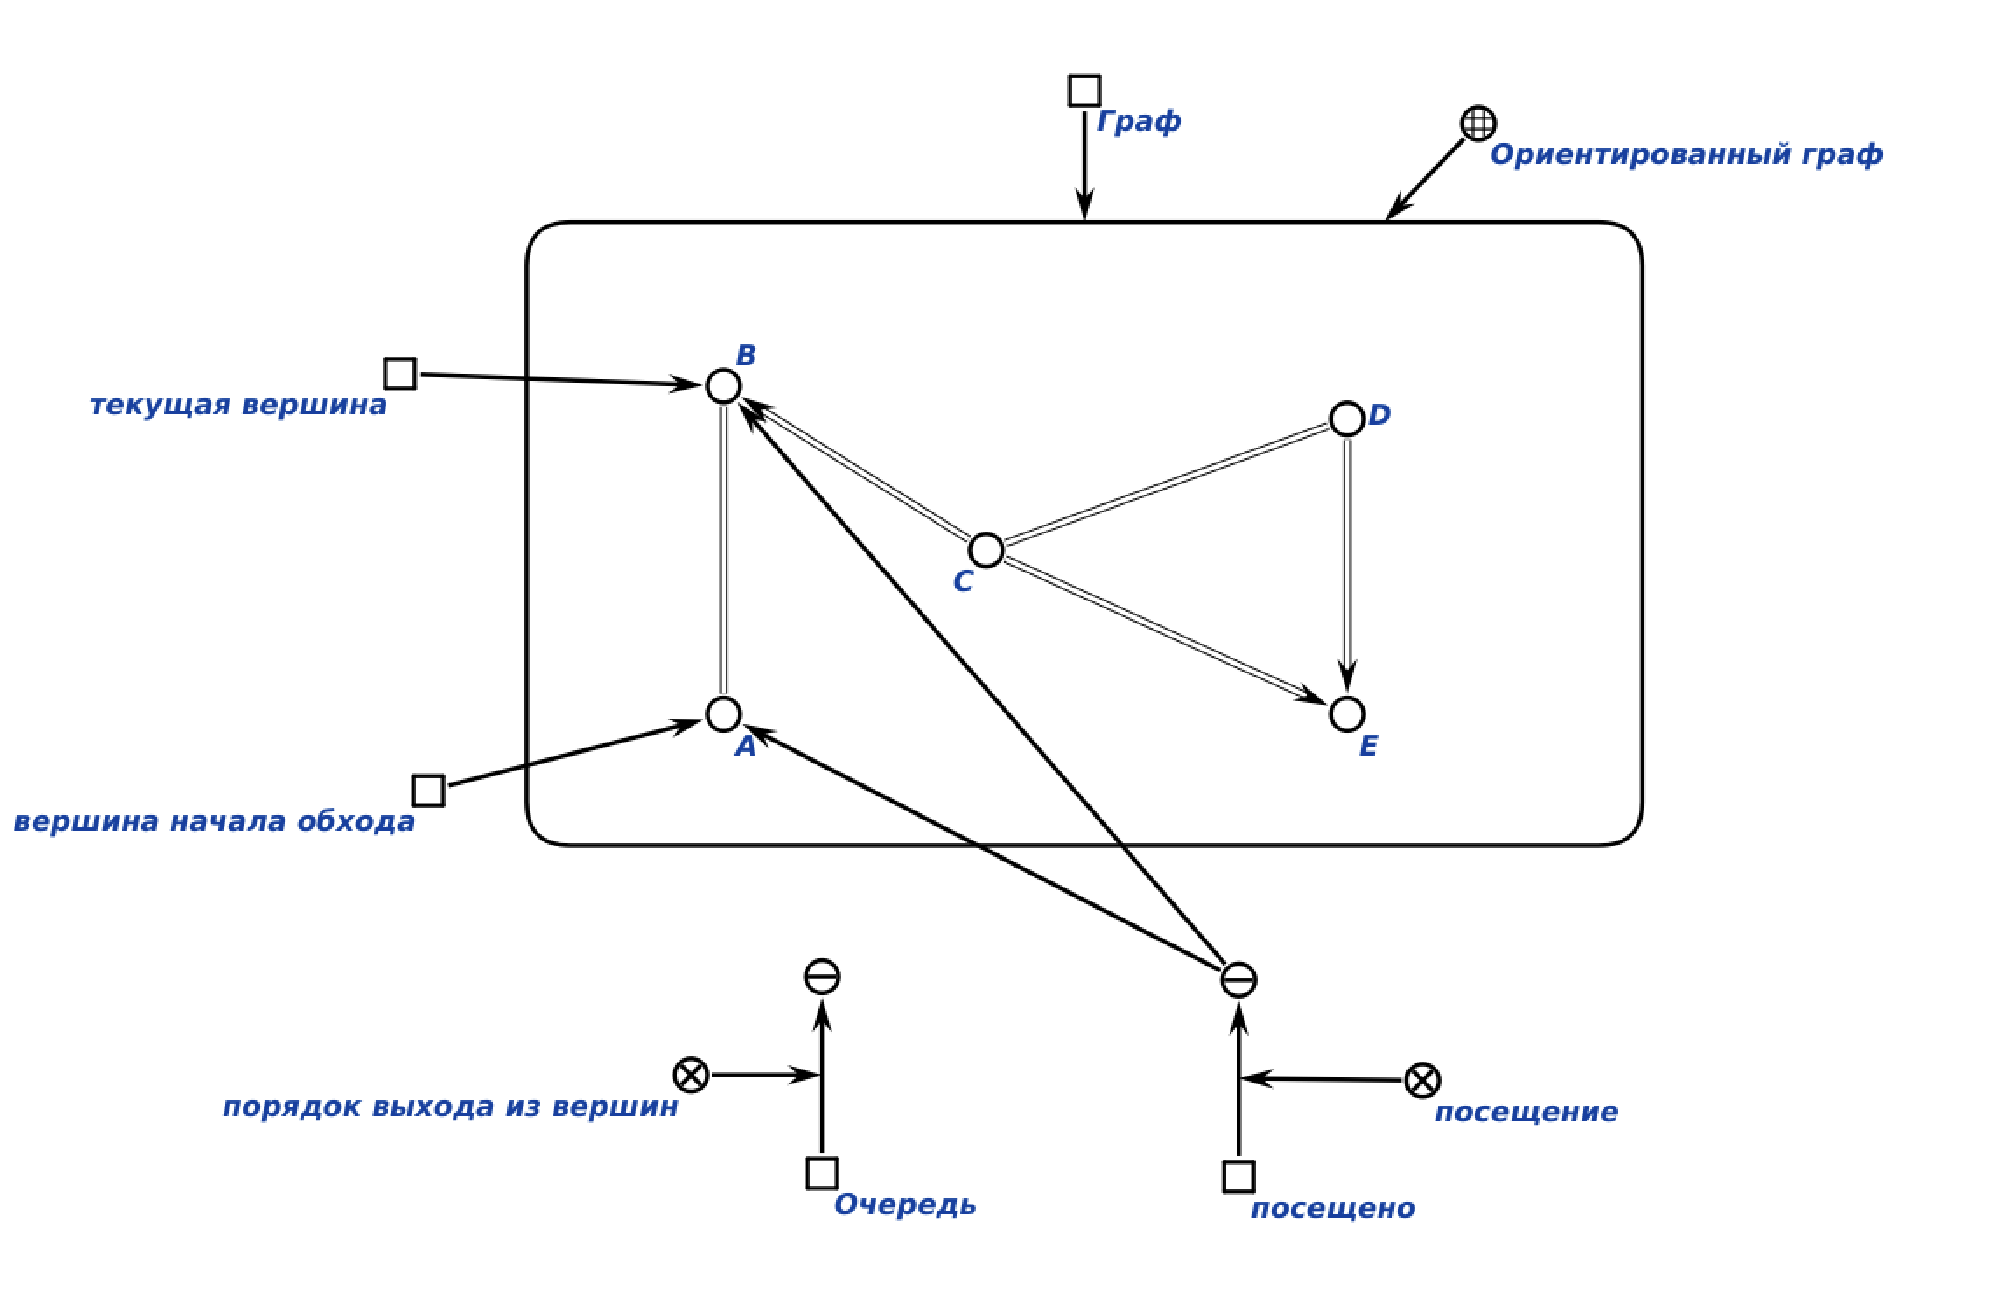
\includegraphics[width=0.45\textwidth]{img/4.png}
		\caption{Рис.4}
	\end{figure}
    \newpage
% 5
	\item Помечаем вершину C как посещённую.
	\begin{figure}[h]
		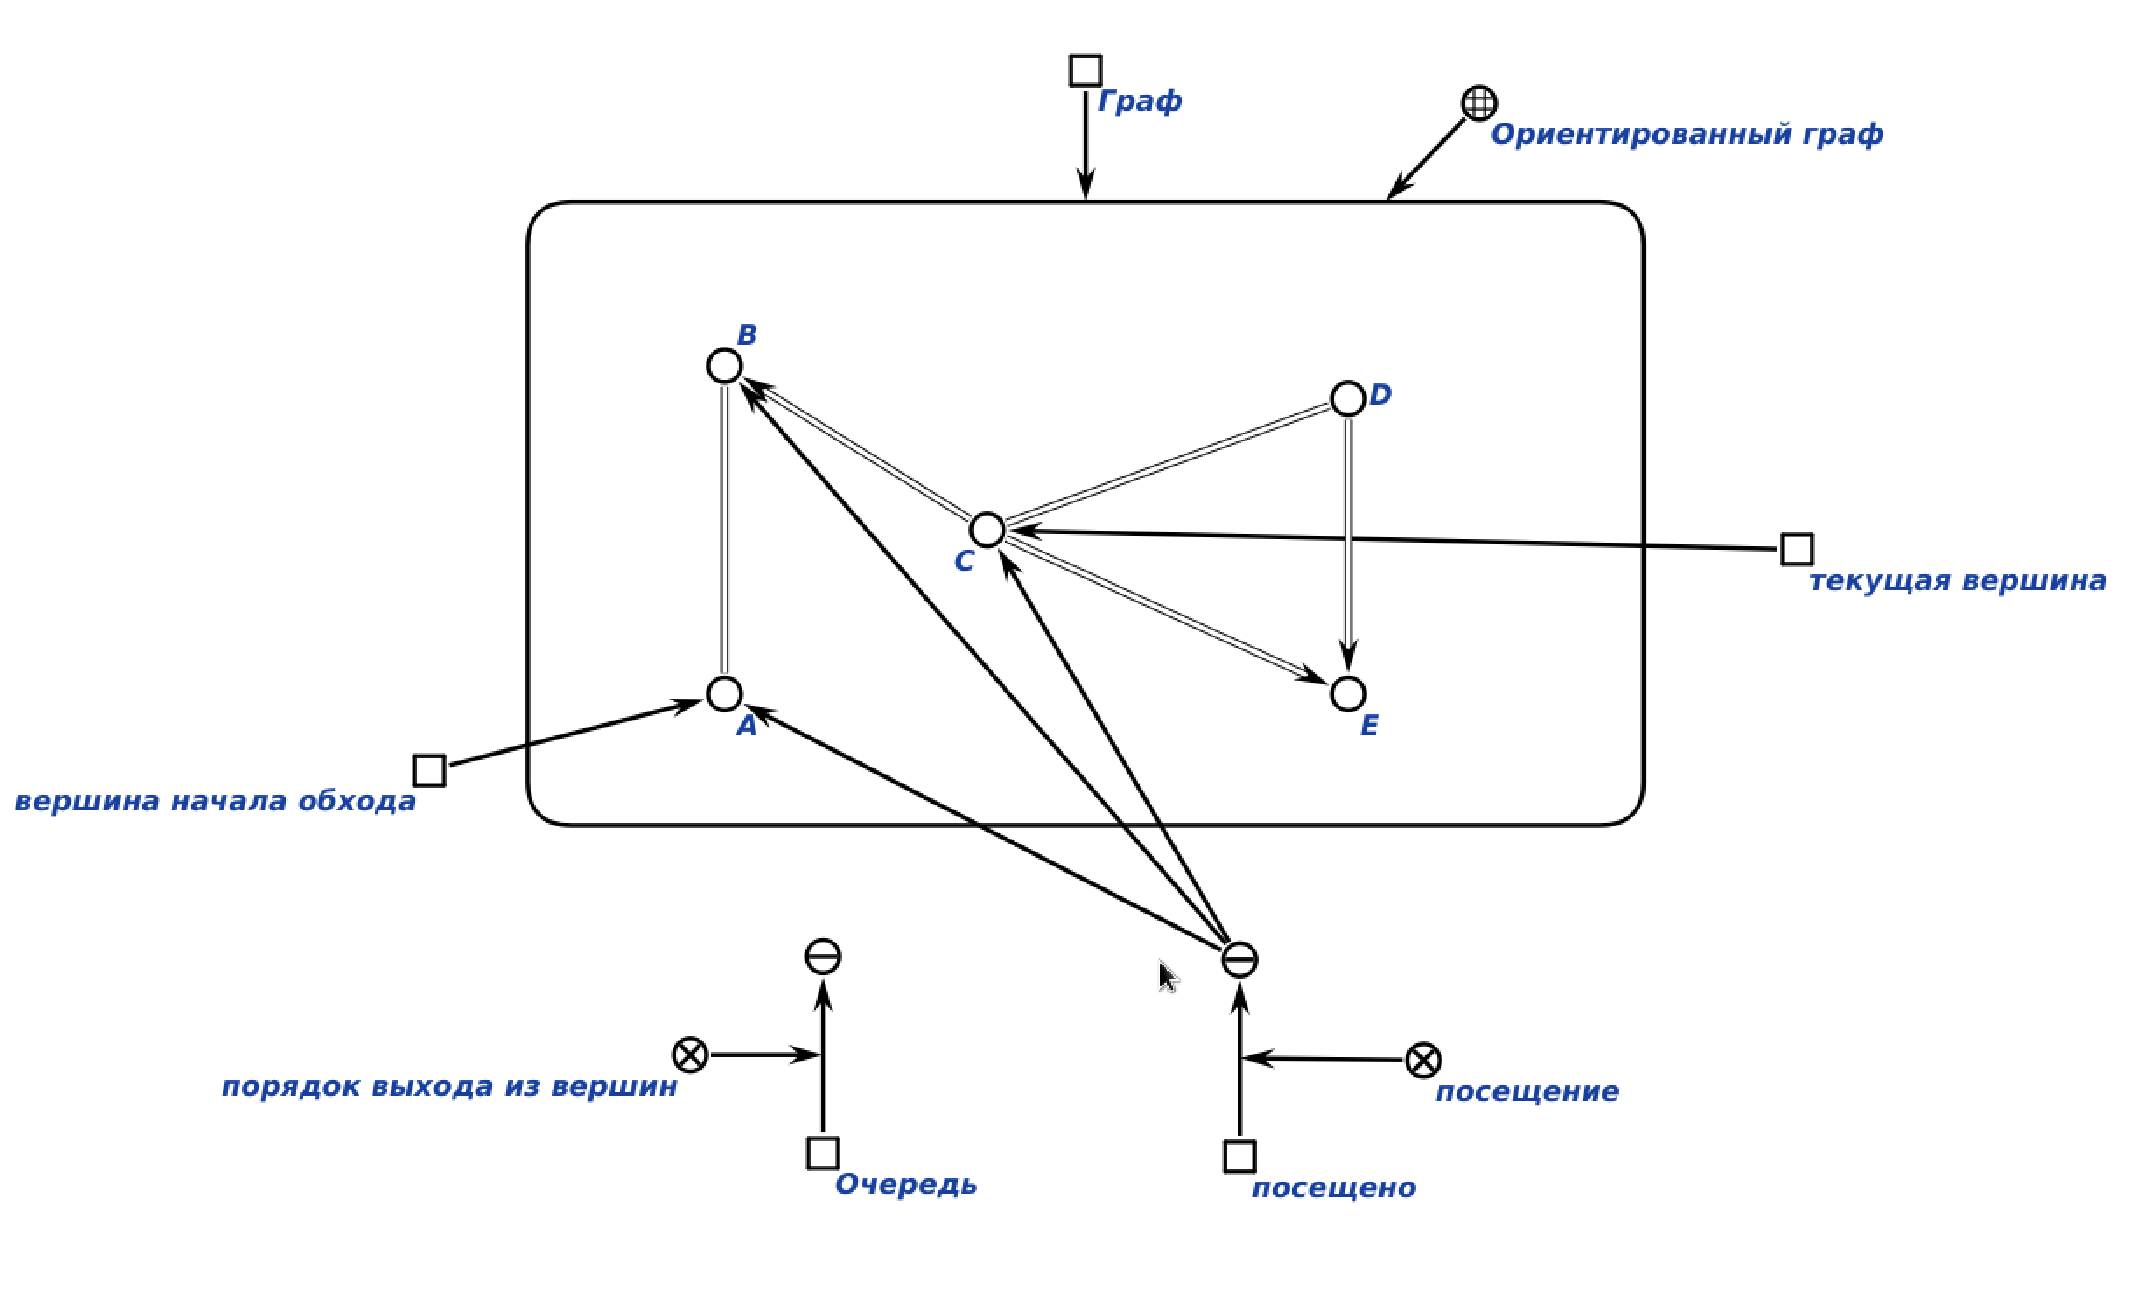
\includegraphics[width=0.45\textwidth]{img/5.png}
		\caption{Рис.5}
	\end{figure}
% 6
	\item Так как вершина B помечена как посещённая, переходим на вершину D и помечаем её как посещённую.
	\begin{figure}[h]
		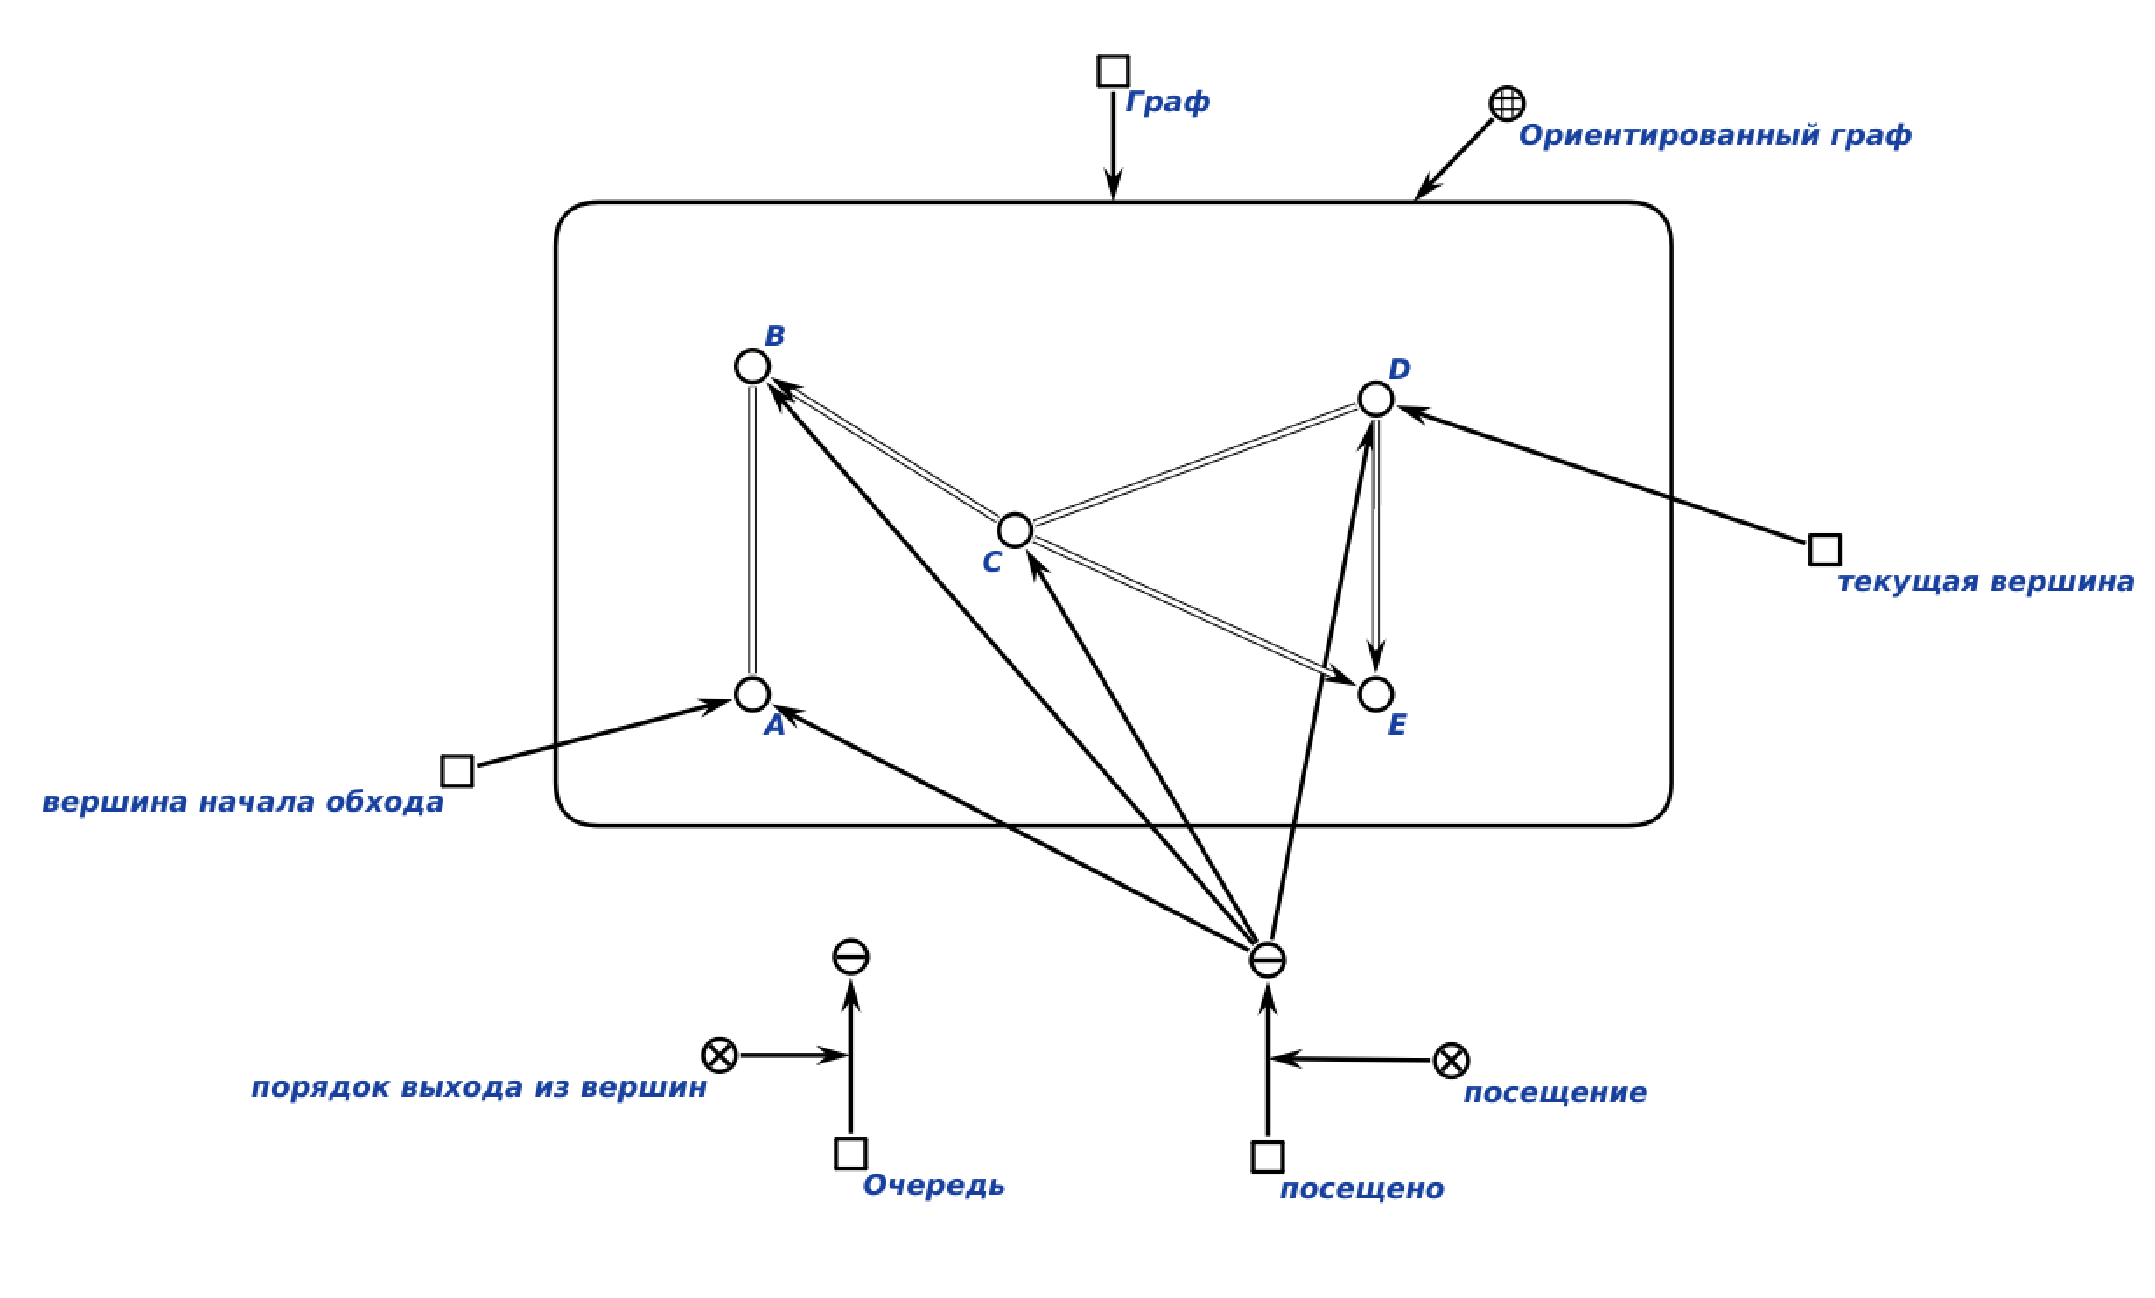
\includegraphics[width=0.45\textwidth]{img/6.png}
		\caption{Рис.6}
	\end{figure}
% 7
	\item Помечаем вершину E как посещённую.
	\begin{figure}[h]
		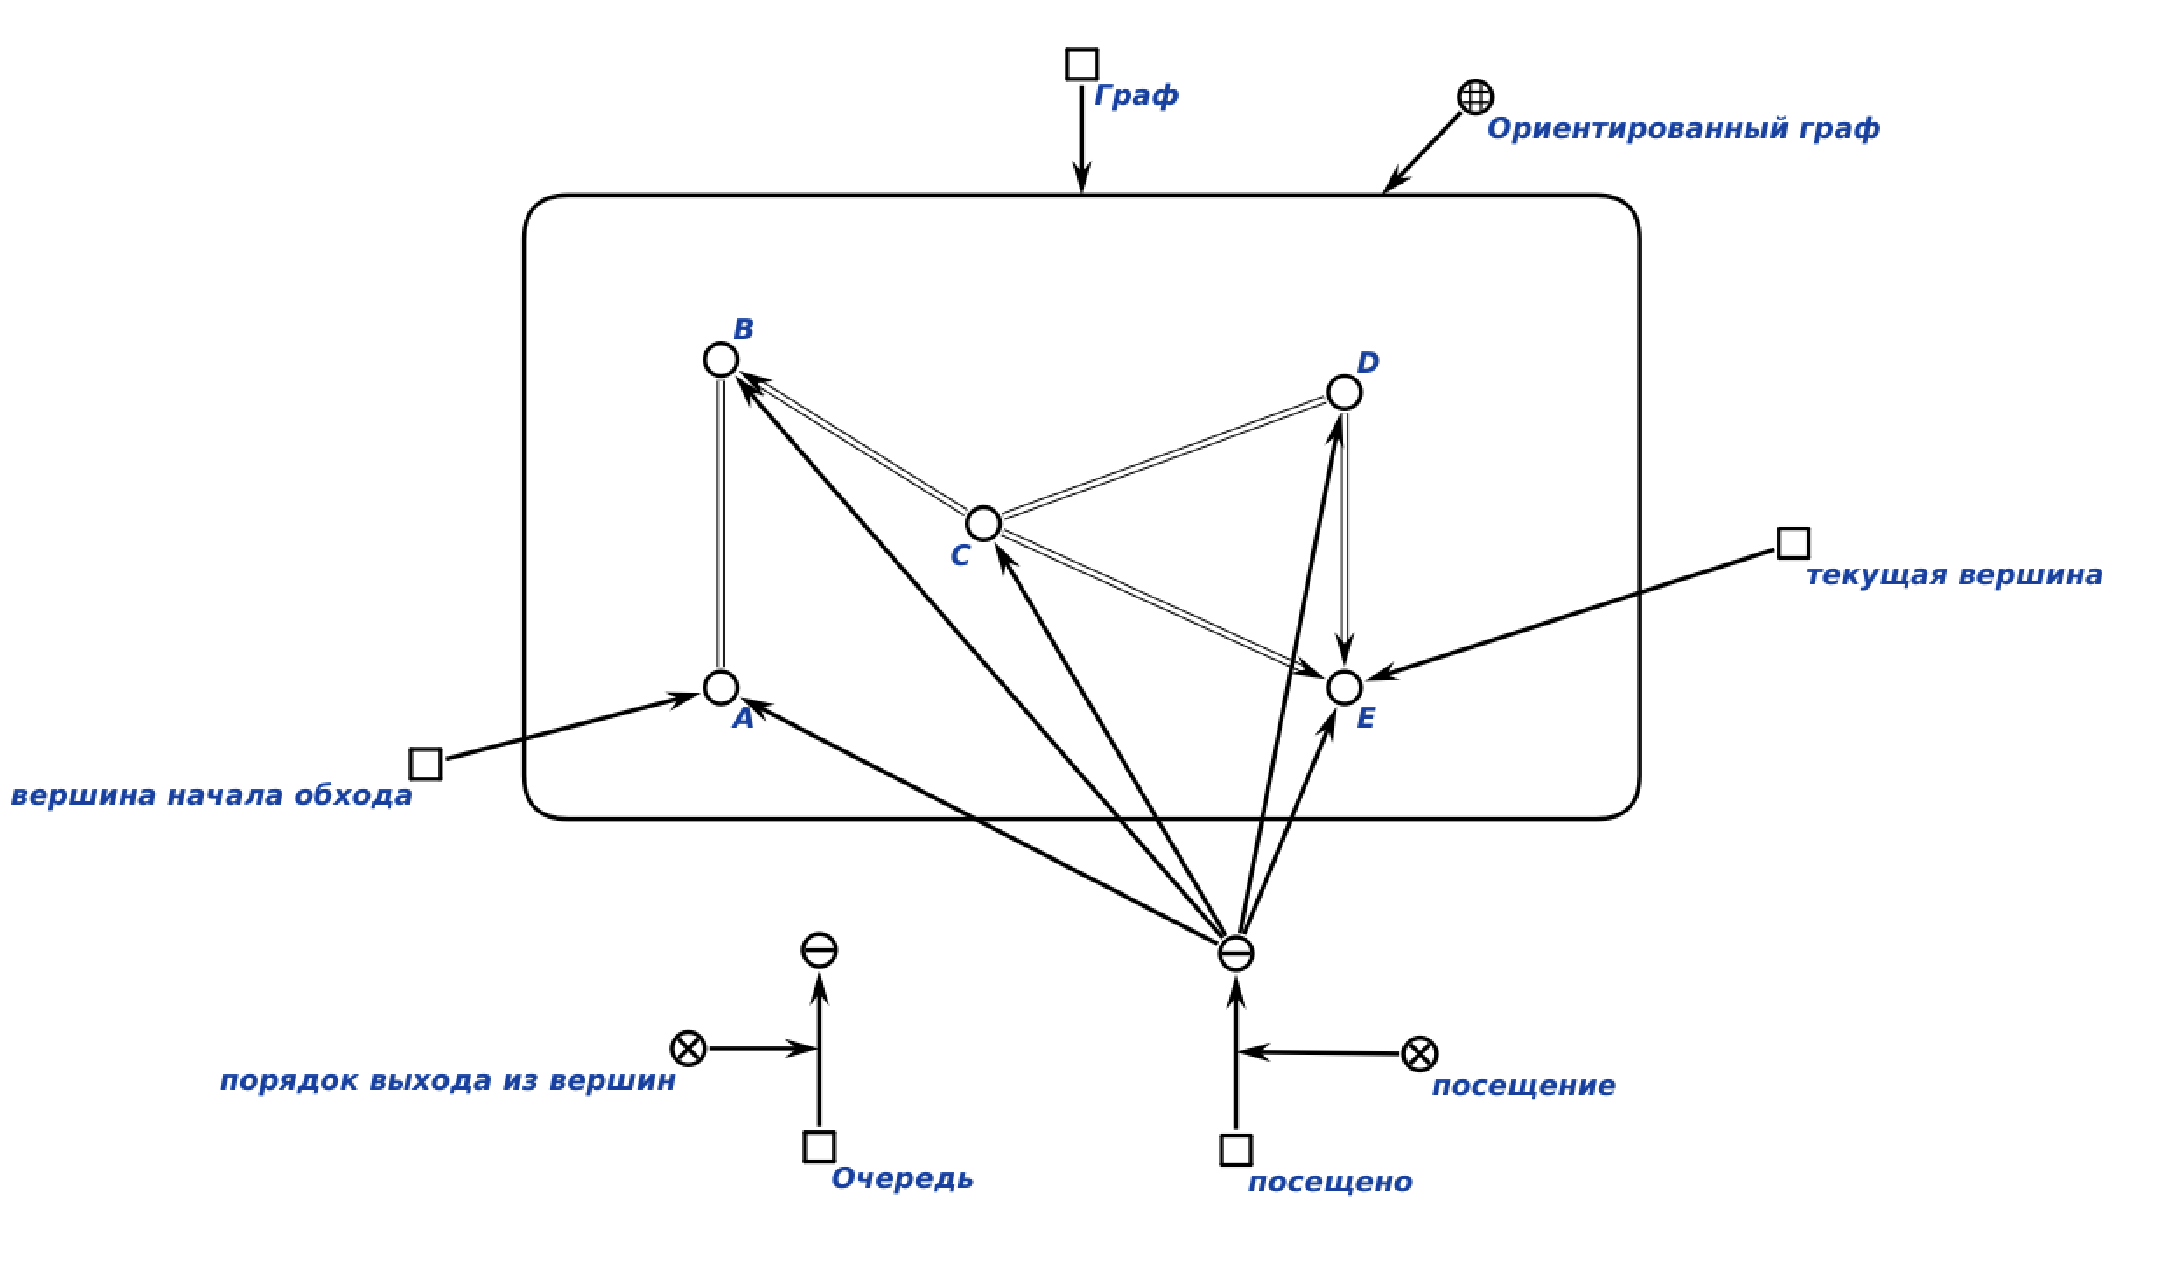
\includegraphics[width=0.45\textwidth]{img/7.png}
		\caption{Рис.7}
	\end{figure}
    \newpage
% 8
	\item Так как все вершины посещены, сохраняем обратный порядок посещения вершин в очередь.
    \begin{figure}[h]
		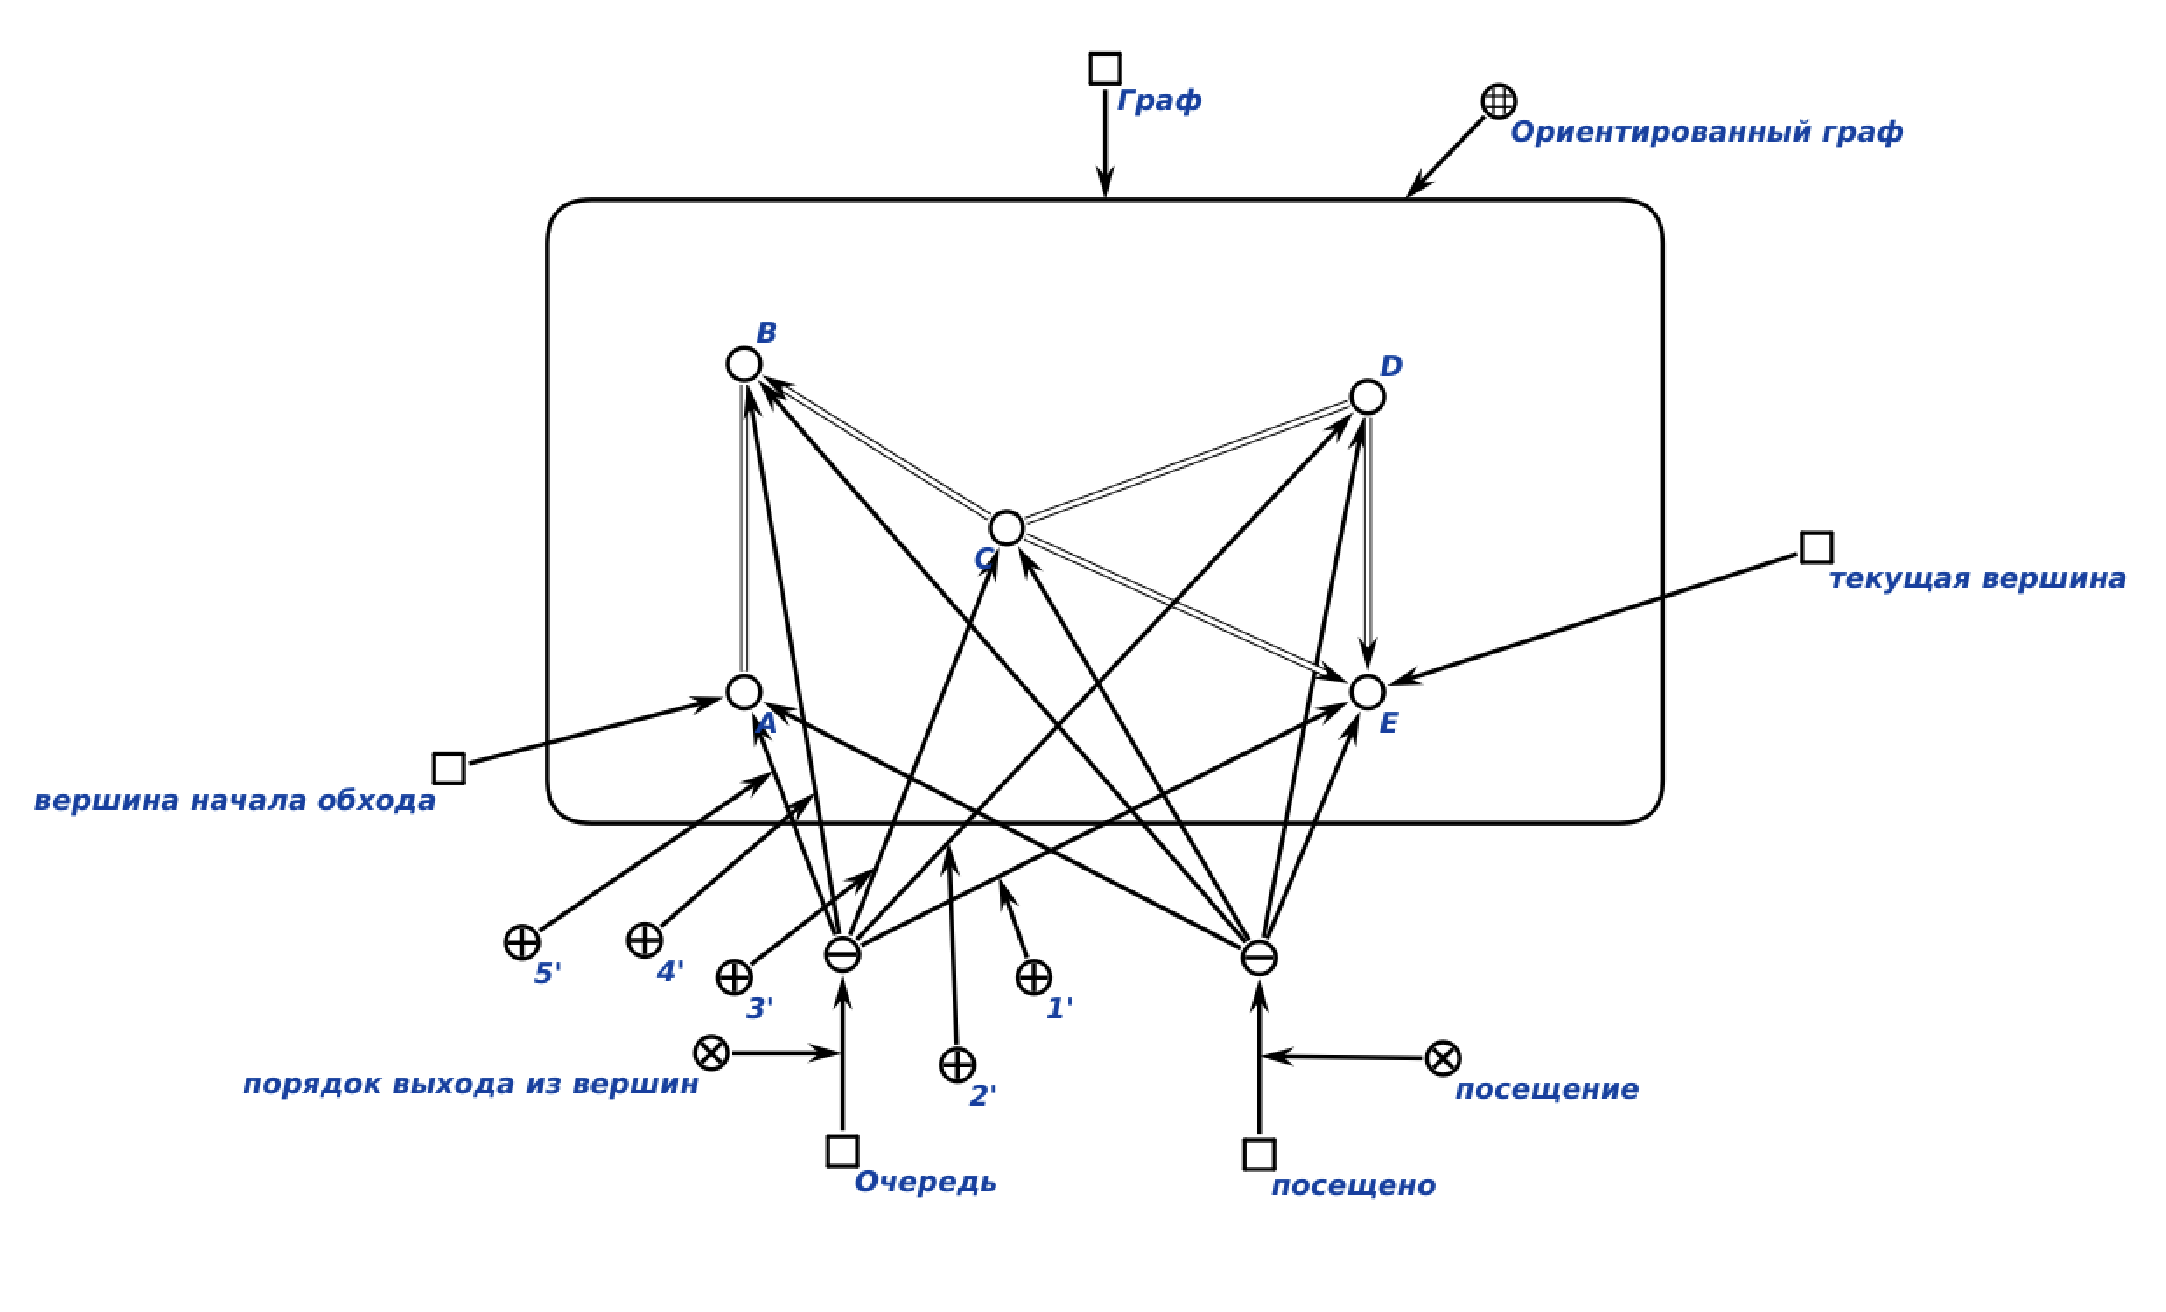
\includegraphics[width=0.45\textwidth]{img/8.png}
		\caption{Рис.8}
	\end{figure}
% 9
	\item Меняем направление всех рёбер на противоположные, т. е. транспонируем граф.
	\begin{figure}[h]
		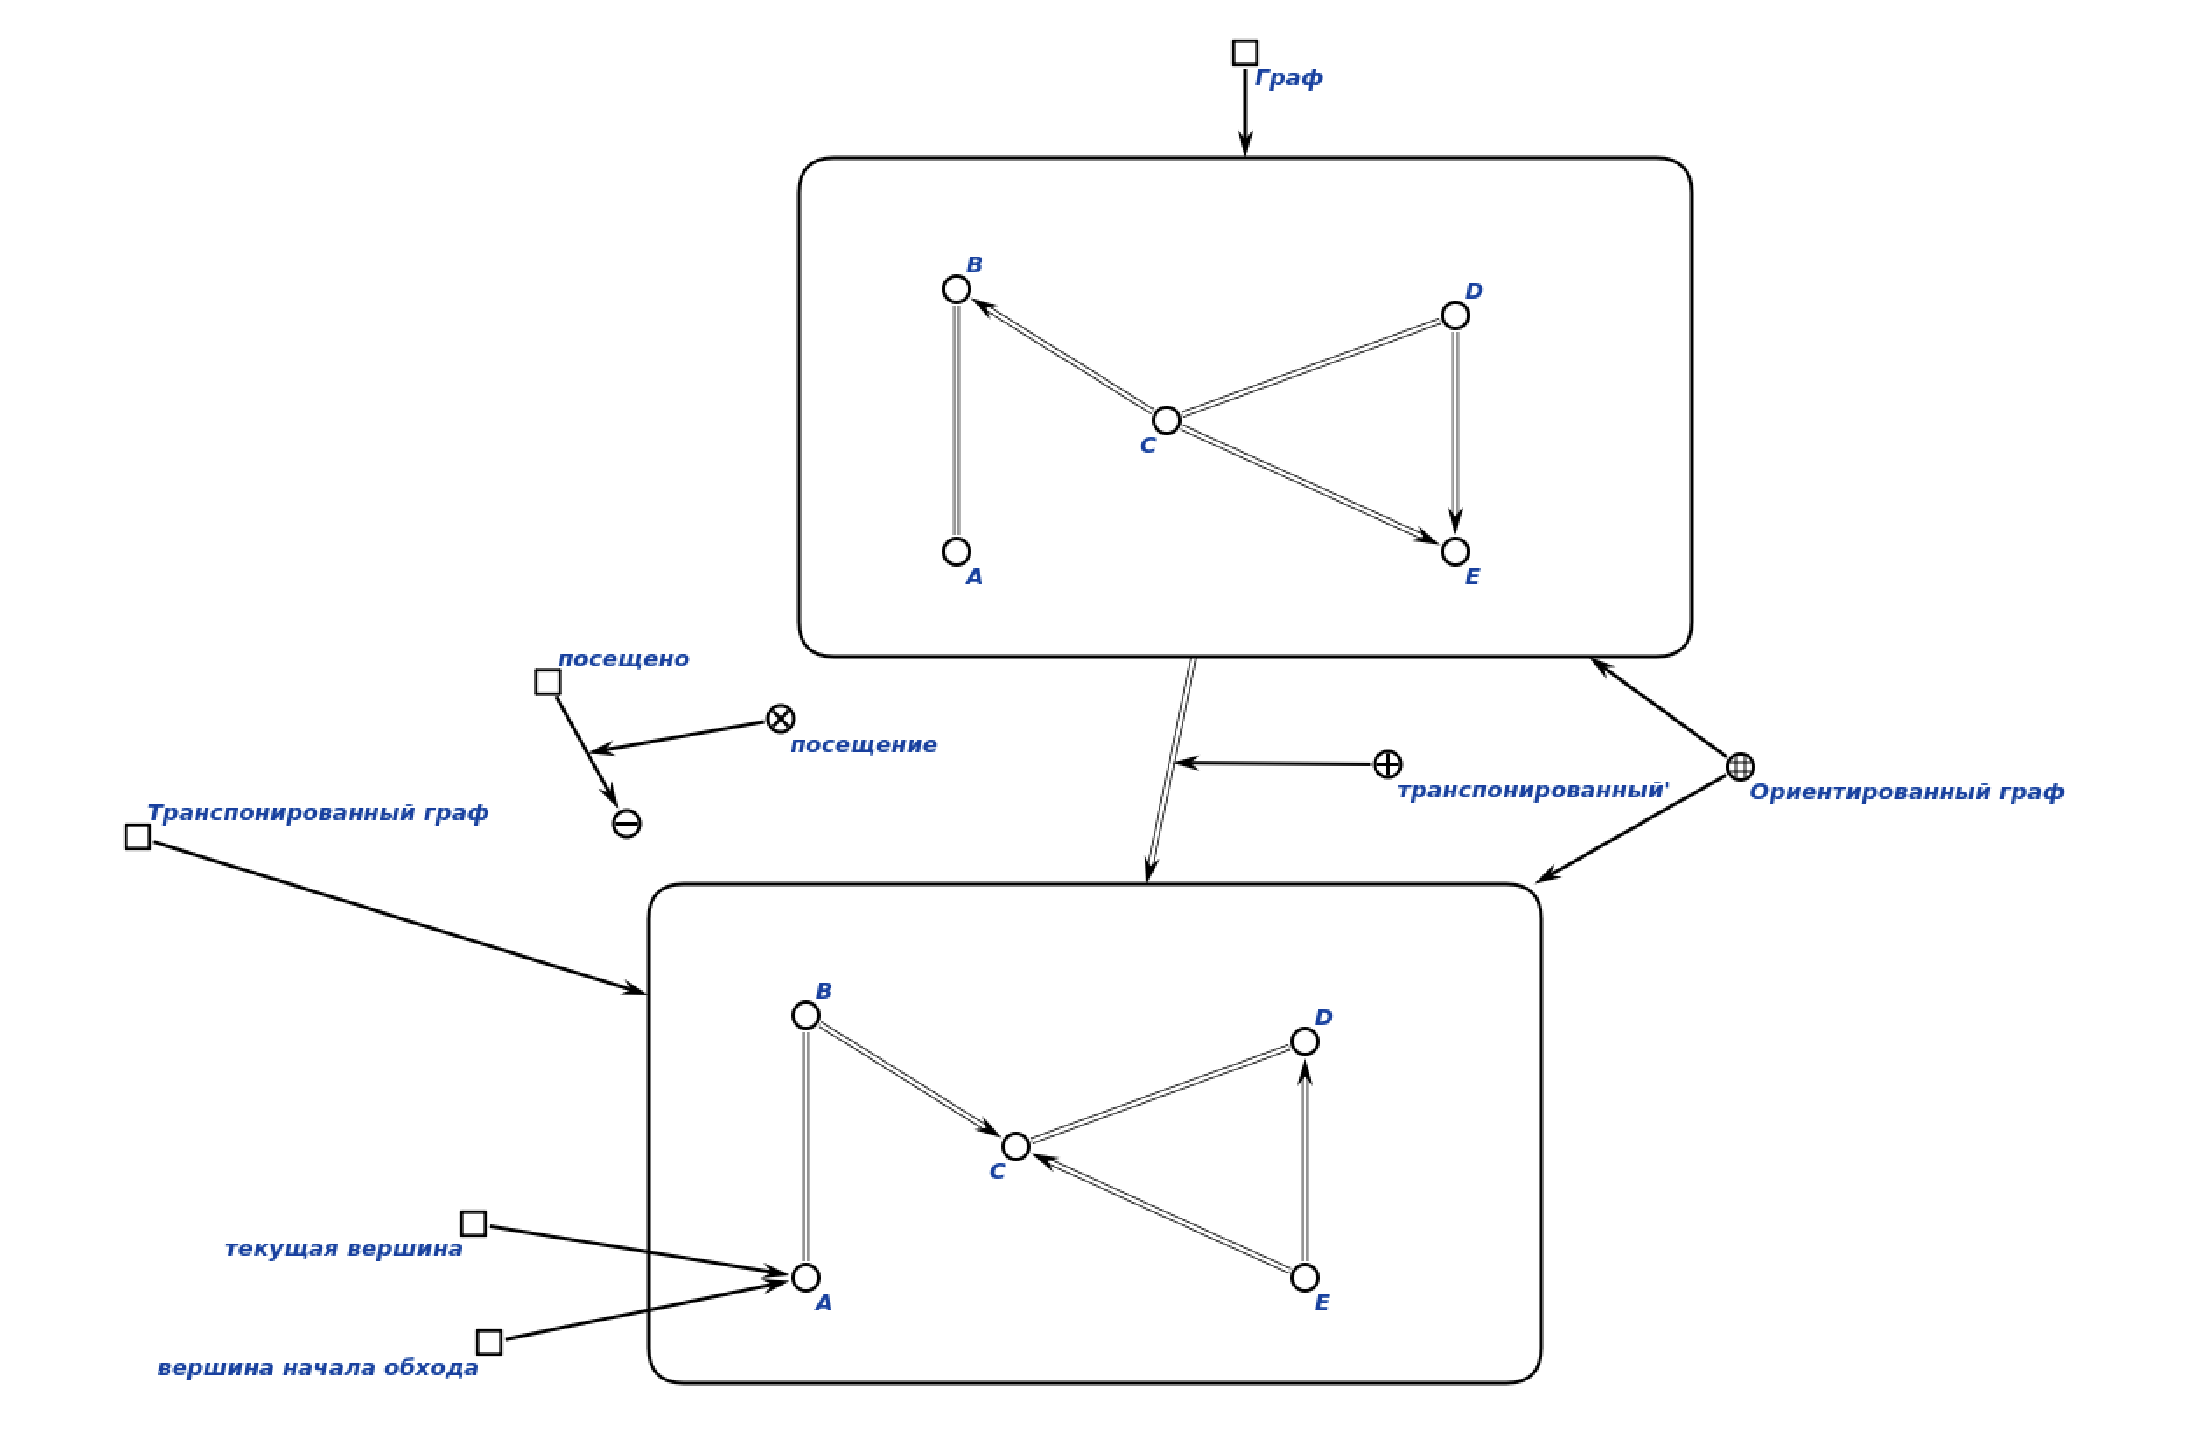
\includegraphics[width=0.45\textwidth]{img/9.png}
		\caption{Рис.9}
	\end{figure}
% 10
	\item Начинаем обход в глубину, начиная с вершины, из которой мы вышли последней. Создаём новый граф. При нахождении новой компоненты сильной связи, добавляем её в новый граф в виде нового узла. Помечаем вершину E как посещённую.
	\begin{figure}[h]
		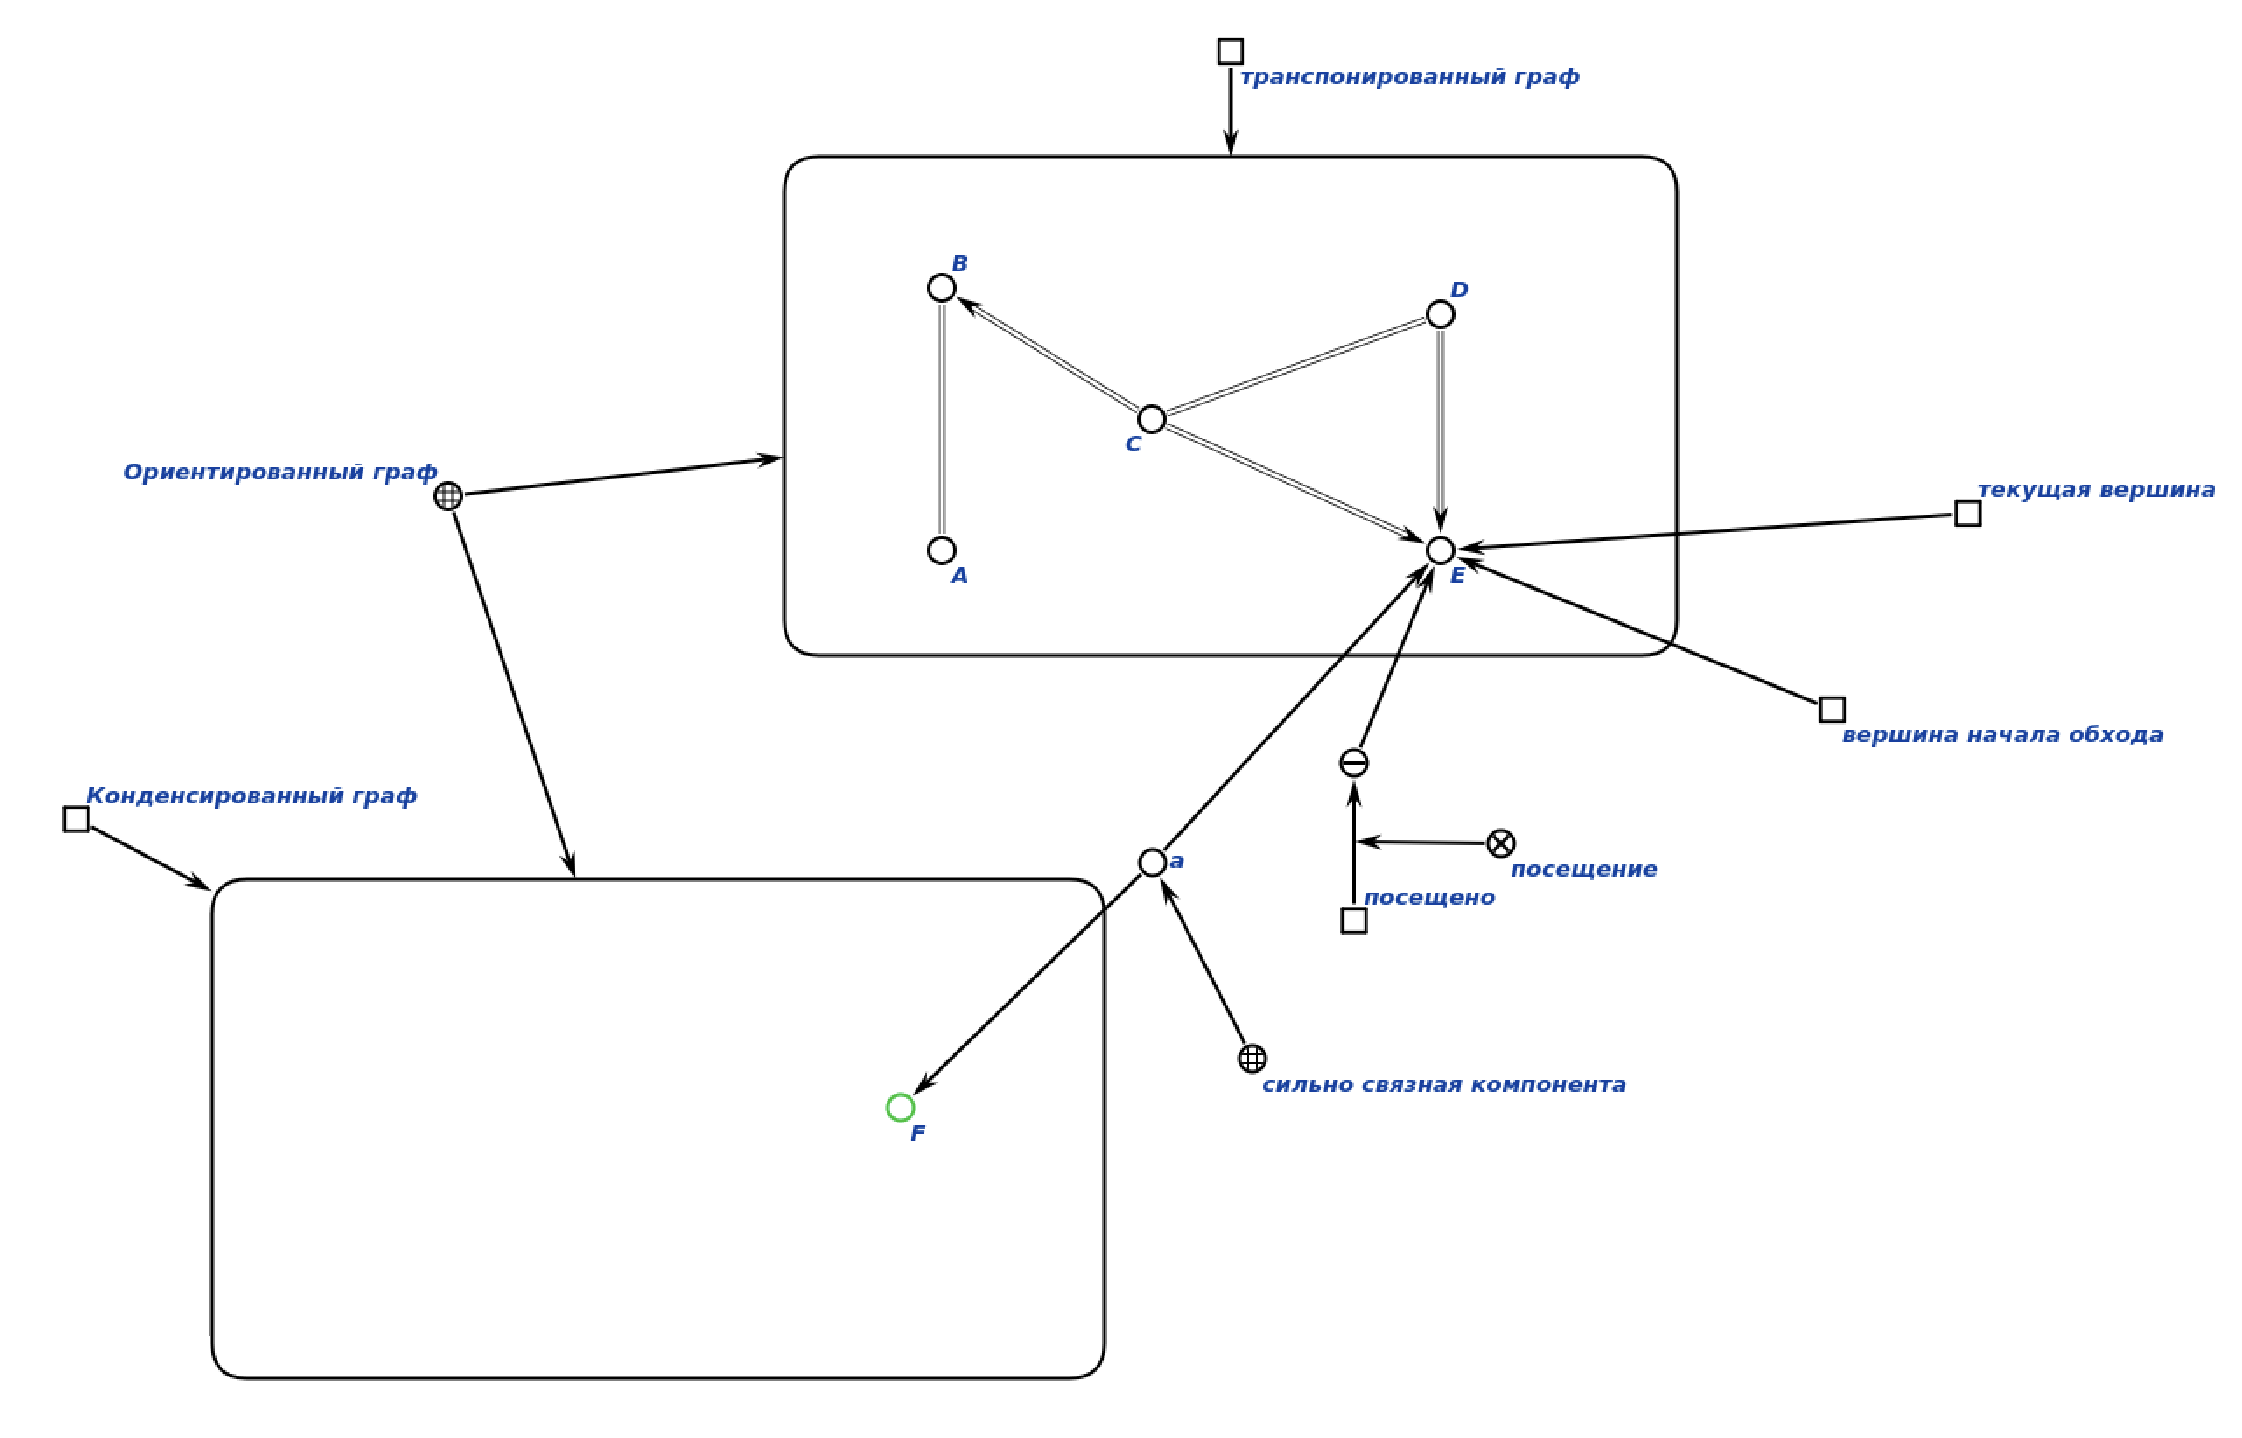
\includegraphics[width=0.45\textwidth]{img/10.png}
		\caption{Рис.10}
	\end{figure}
    \newpage
% 11
	\item Помечаем вершину D как посещённую. Так как из D нельзя попасть в E, создаём новую сильную компоненту b и  вершину G в сконденсированном графе. Сохраняем отношения между сильными компонентами.
	\begin{figure}[h]
		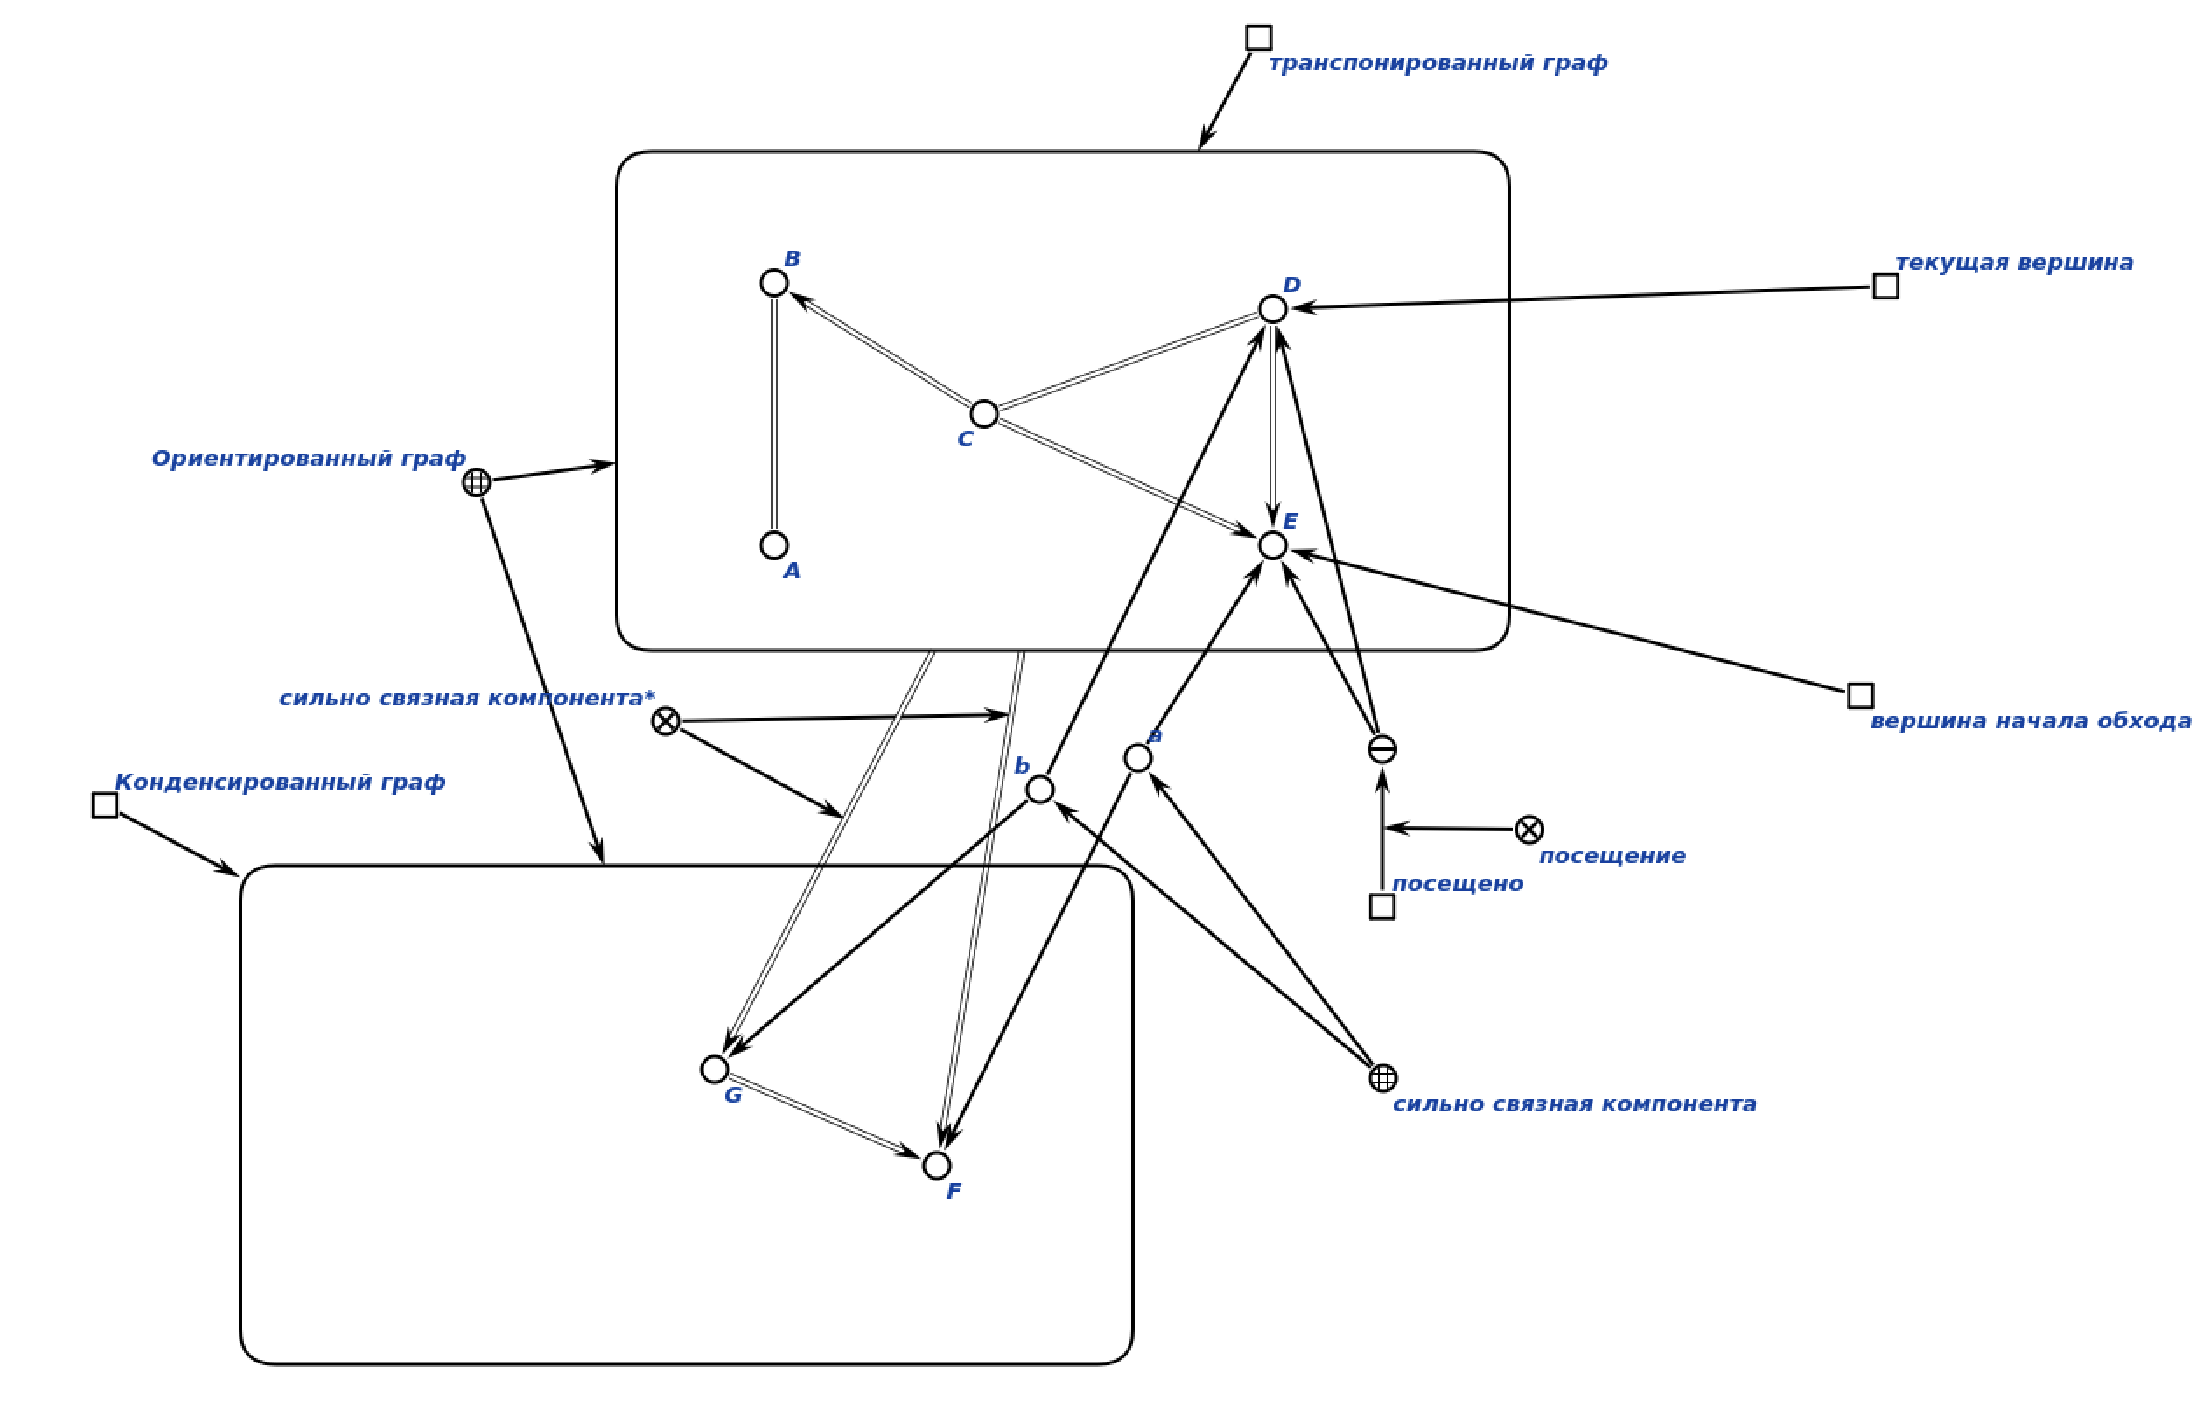
\includegraphics[width=0.45\textwidth]{img/11.png}
		\caption{Рис.11}
	\end{figure}
% 12
	\item Помечаем вершину C как посещённую. Так как из вершины C можно попасть в D, добавляем вершину C в сильную компоненту b, а её в вершину G.
	\begin{figure}[h]
		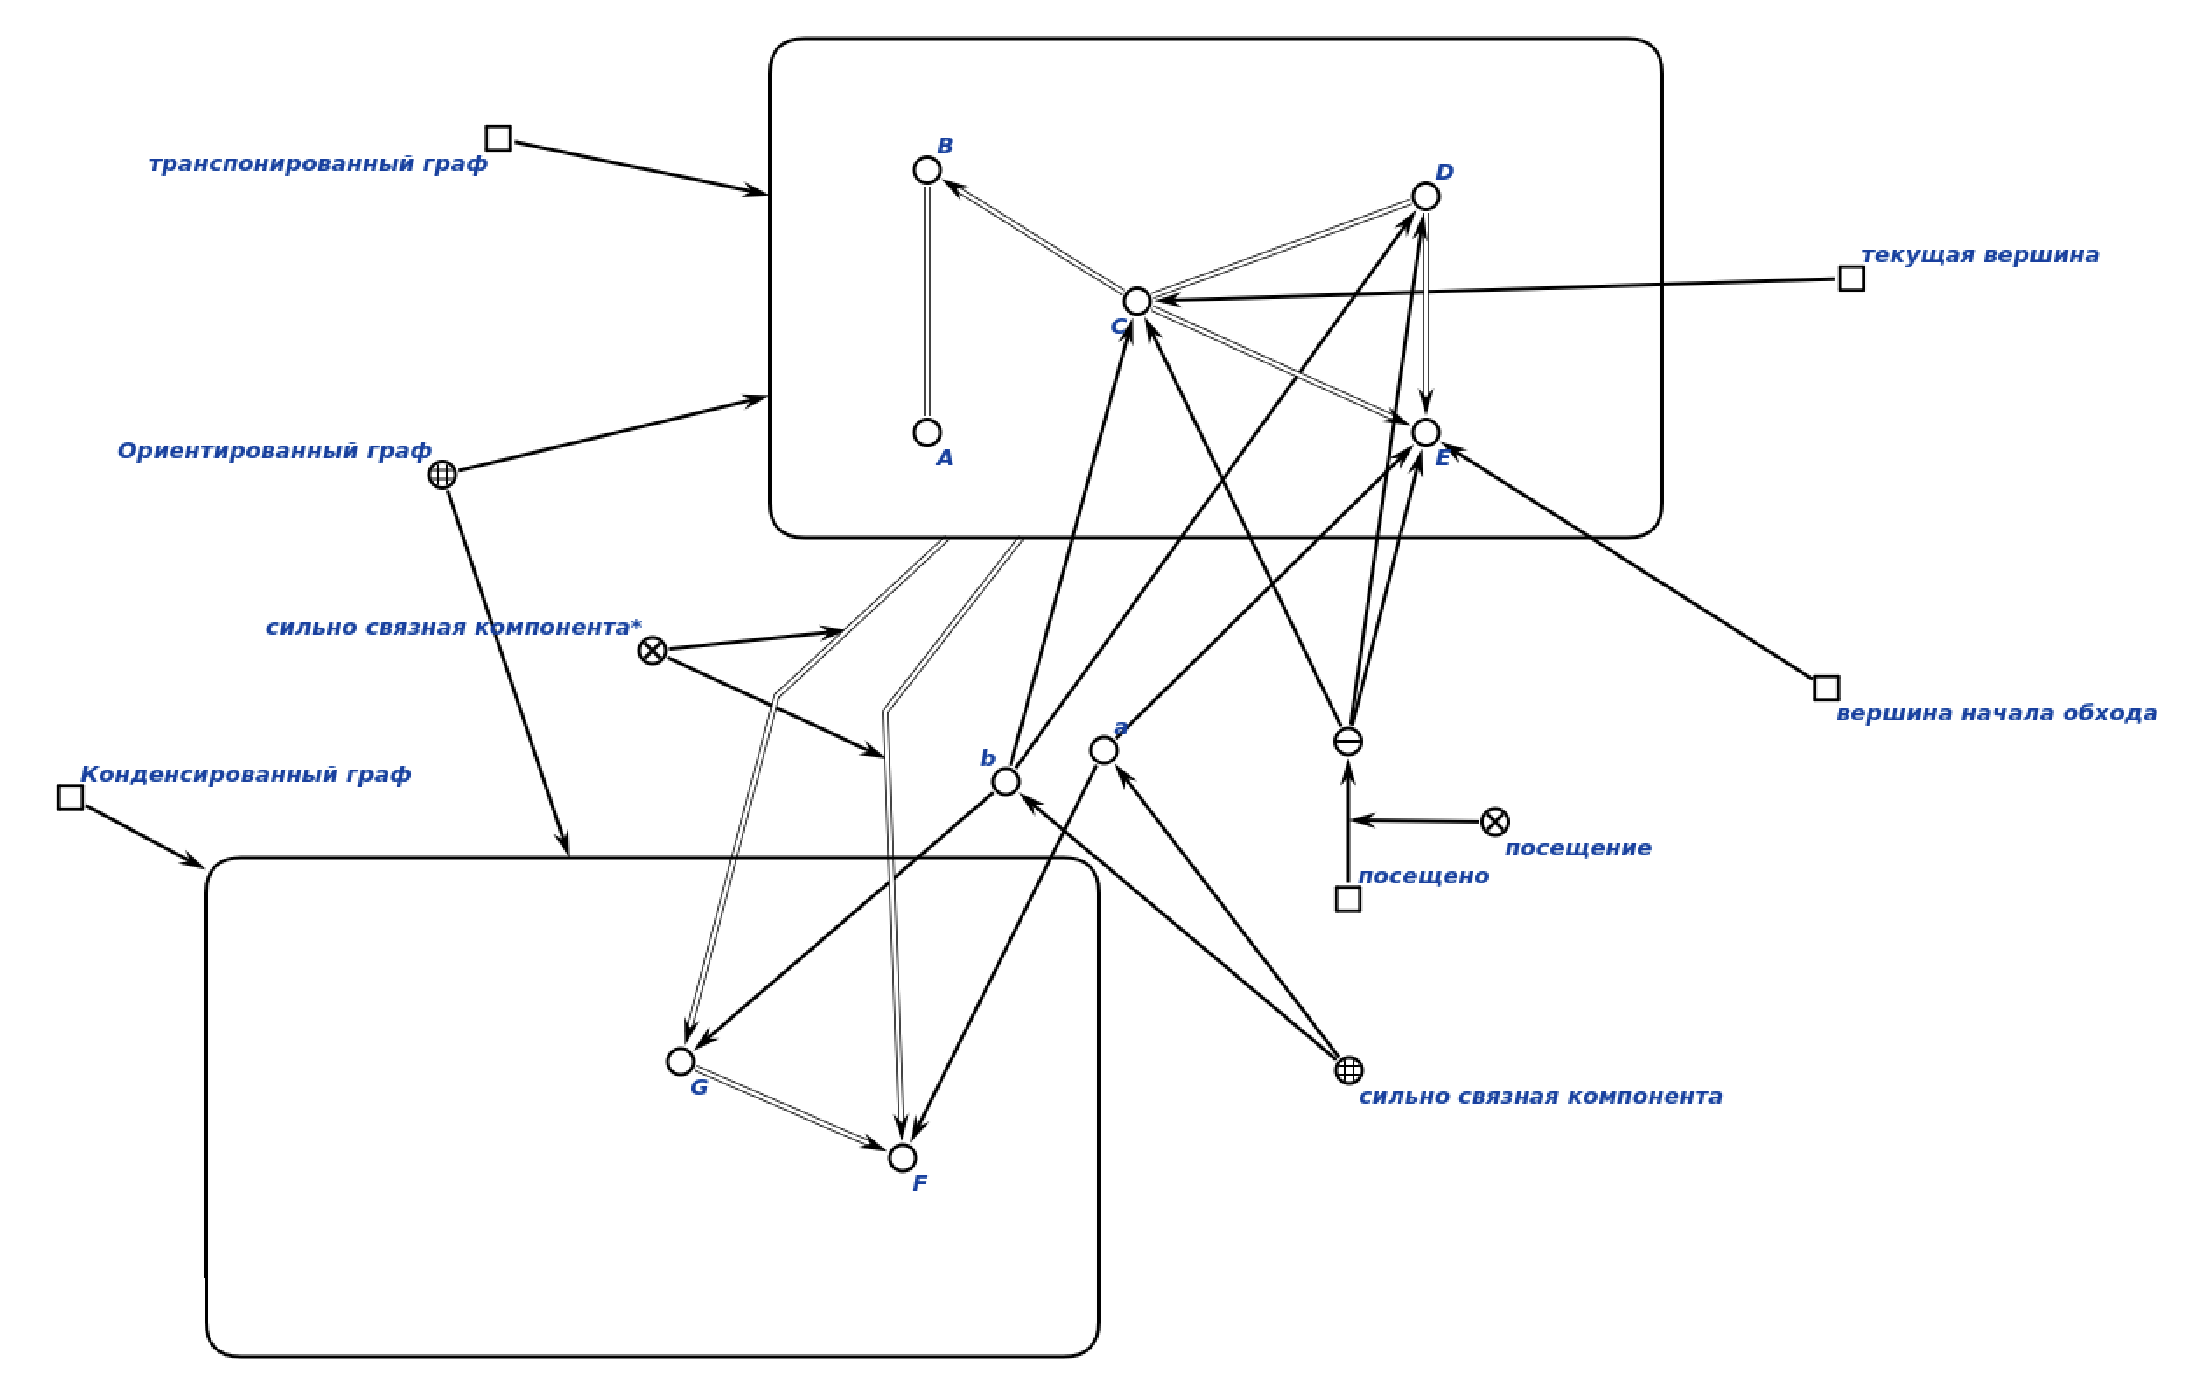
\includegraphics[width=0.45\textwidth]{img/12.png}
		\caption{Рис.12}
	\end{figure}
% 13
	\item Помечаем вершину B как посещённую. Так как в C мы не можем попасть из B, создаём новую сильную компоненту c и новую вершину H в конденсированном графе.
	\begin{figure}[h]
		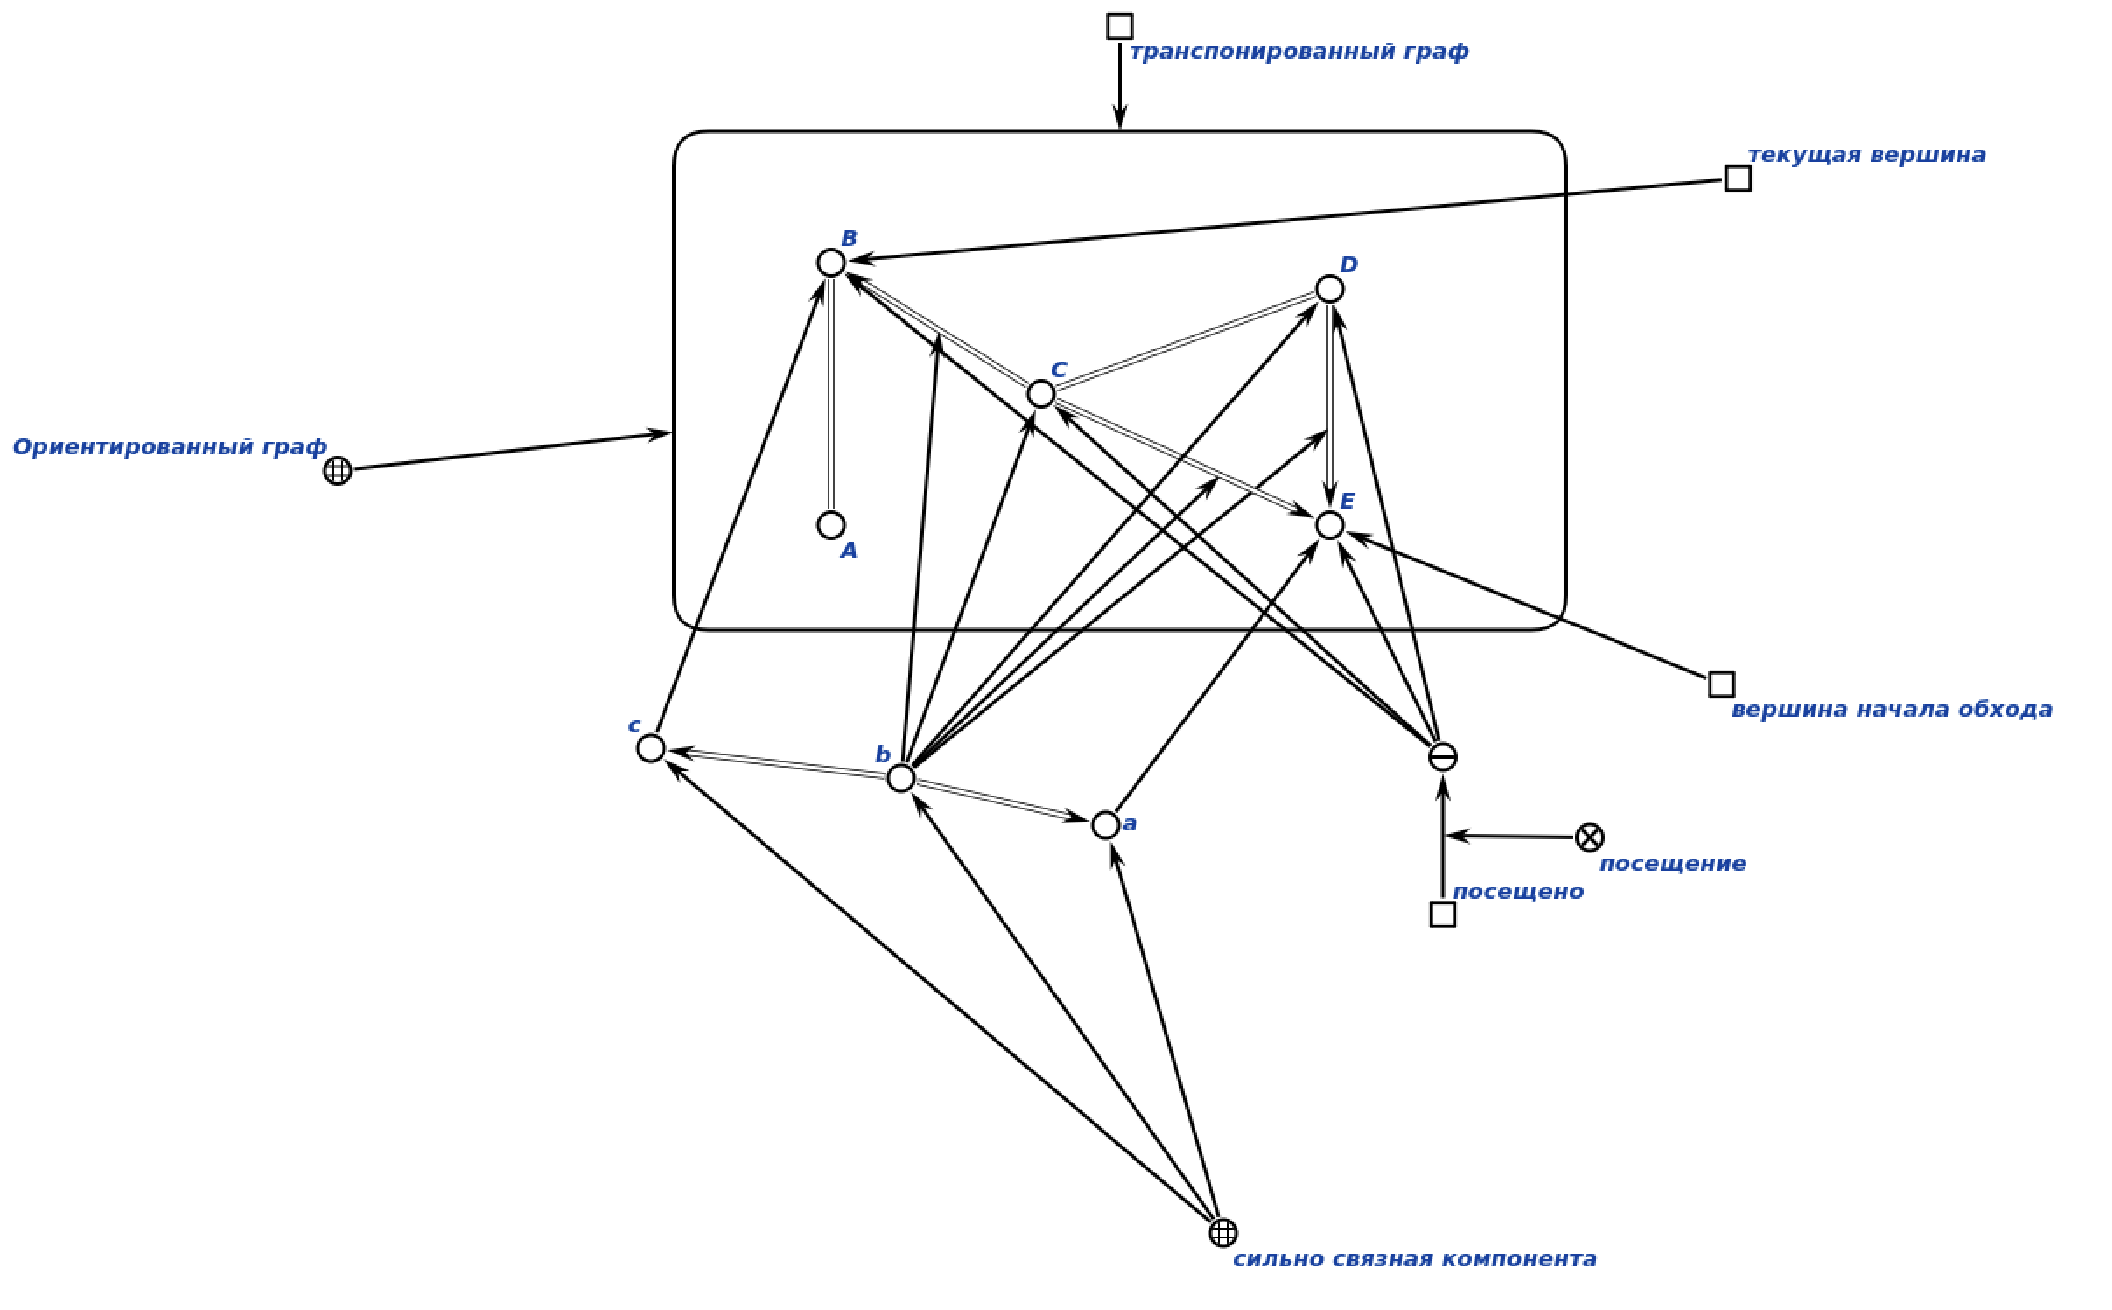
\includegraphics[width=0.45\textwidth]{img/13.png}
		\caption{Рис.13}
	\end{figure}
% 14
	\item Помечаем вершину A как посещённую. Так как из вершины A можно попасть в B, добавляем вершину A в сильную компоненту c, а её в вершину G.
	\begin{figure}[h]
		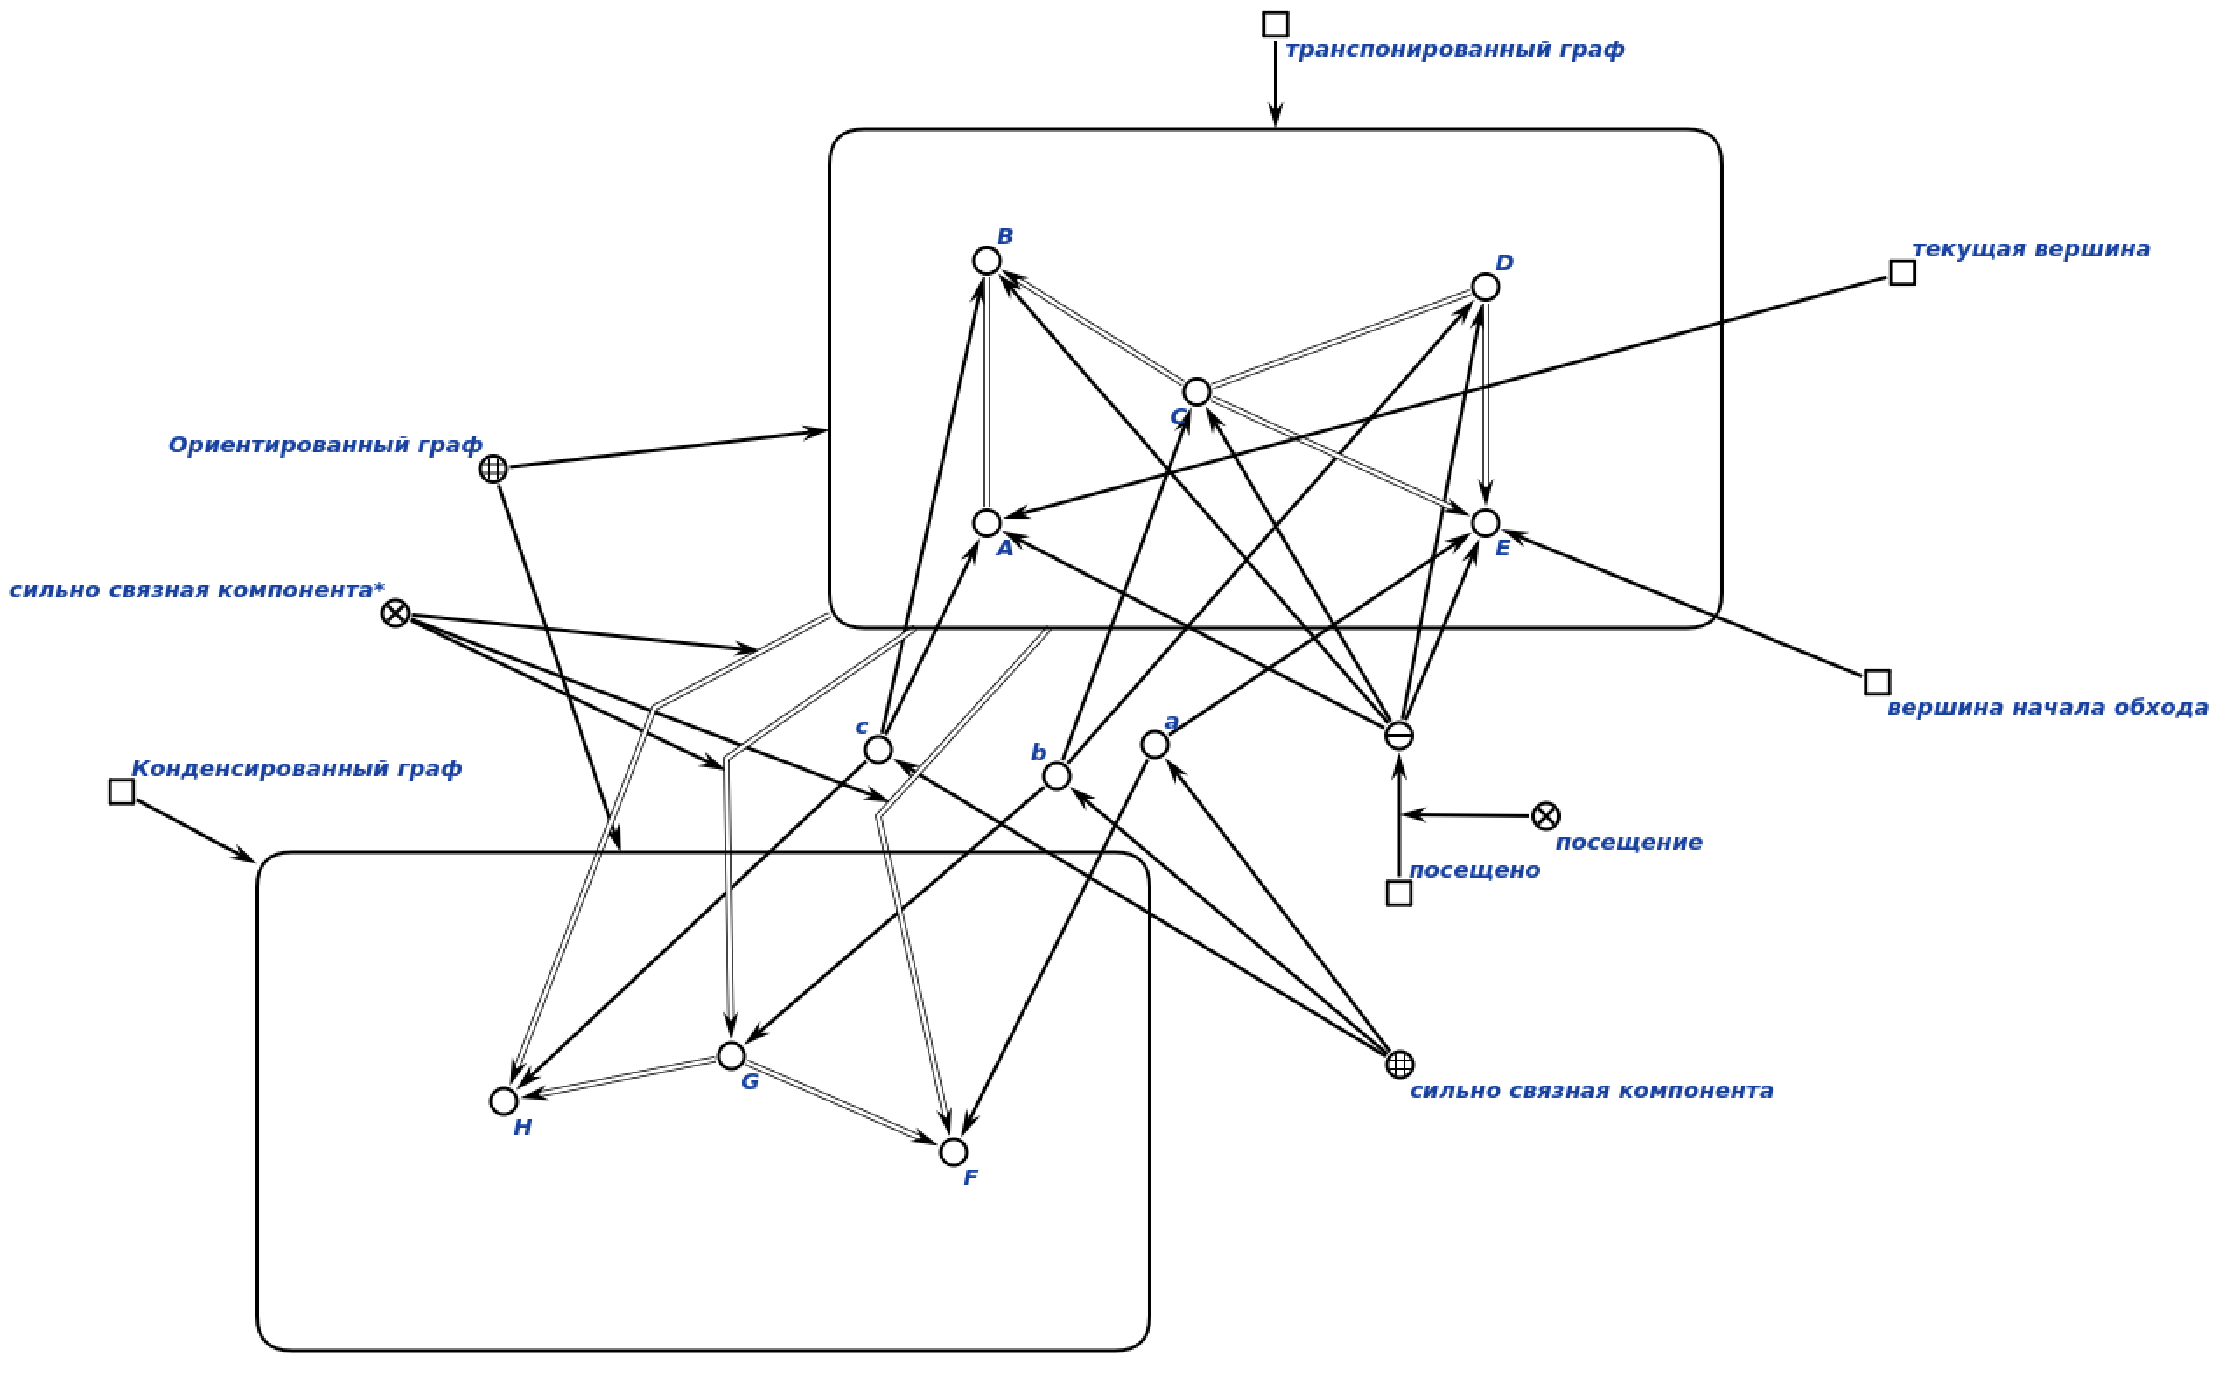
\includegraphics[width=0.45\textwidth]{img/14.png}
		\caption{Рис.14}
	\end{figure}
\end{enumerate}
\large{\textbf{Выводы:}}
\par В результате выполнения данной расчётной работы был формализован алгоритм нахождения конденсированного графа из ориентированного, были изучены:
\begin{enumerate}
	\item[$\bullet$] Основы теории графов
	\item[$\bullet$] Способы представления графов
	\item[$\bullet$] Базовые алгоритмы для работы с графами
	\item[$\bullet$] Основы SC-кода и SC-алфавита
\end{enumerate}
\large{\textbf{Источники:}}
\begin{enumerate}
	\item[$\bullet$] Оре О. Теория графов. – 2-е изд.. – М.: Наука, 1980. – С. 336.
	\item[$\bullet$] Кормен Т. Х. и др. Часть VI. Алгоритмы для работы с графами // Алгоритмы: построение и анализ = Introduction to Algorithms. – 2-е изд.. – М.: Вильямс, 2006. – С. 1296.
	\item[$\bullet$] Харари, Ф. Теория графов / Ф. Харари / Пер. с англ. и предисл. В.П. Козырева. Под ред. Г.П. Гаврилова. Изд. 2-е. – М.: Едиториал УРСС, 2003. – 269 с.
    \item[$\bullet$]  wikipedia.org
\end{enumerate}
\end{document}